\documentclass[a4paper, 11pt, notitlepage,english]{article}

%
% Importering av pakker
%
\usepackage[utf8]{inputenc}
\usepackage[english]{babel}
\usepackage{lmodern}
\usepackage{algorithm,algorithmic}
\usepackage[T1]{fontenc, url}
\usepackage{textcomp}
\usepackage{amsmath, amssymb}
\usepackage{amsbsy, amsfonts}
\usepackage{graphicx, color}
\usepackage{listings}
\usepackage{multicol}
\usepackage{booktabs}
\usepackage{bbm}
\usepackage{amsthm}
\usepackage[text={6.2in,9.2in},centering]{geometry}
\usepackage{subfigure}
\bibliographystyle{plain}
 
\definecolor{dkgreen}{rgb}{0,0.6,0}
\definecolor{gray}{rgb}{0.95,0.95,0.95}
\definecolor{mauve}{rgb}{0.58,0,0.82}
 
\usepackage{parskip}
% \usepackage{tabularx}

%
% Parametere for inkludering av kode fra fil
%
%\lstset{language=python}
%\lstset{basicstyle=\ttfamily\small}
%\lstset{frame=single}
%\lstset{keywordstyle=\color{red}\bfseries}
%\lstset{commentstyle=\itshape\color{blue}}
%\lstset{showspaces=false}
%\lstset{showstringspaces=false}
%\lstset{showtabs=false}
%\lstset{breaklines}

\lstset{ %
    language=C++,
    backgroundcolor=\color{gray},
    basicstyle=\footnotesize,
    frame=bt,
    framexleftmargin=5pt,
    keywordstyle=\bf \color{dkgreen},
    commentstyle=\color{mauve}\slshape,
    breaklines=true
}

%
% Definering av egne kommandoer og miljøer
%
\newcommand{\dd}[1]{\ \text{d}#1}
\newcommand{\f}[2]{\frac{#1}{#2}} 
\newcommand{\beq}{\begin{equation*}}
\newcommand{\eeq}{\end{equation*}}
\newcommand{\bo}[1]{\boldsymbol{#1}}
\newcommand{\BAR}{%
  \hspace{-\arraycolsep}%
  \strut\vrule % the `\vrule` is as high and deep as a strut
  \hspace{-\arraycolsep}%
}
\newcommand{\norm}[1]{\left\lVert #1 \right\rVert}
\newcommand{\id}{\mathbbm{1}}
\newcommand{\idop}{\bbm 1}

\newtheorem{theorem}{Theorem}

%
% Navn og tittel
%
\author{Candidate numbers: 70, 65}
\title{FYS4150 - Computational Physics \\
      Project 5: \\
       Diffusion of neurotransmitters in the synaptic cleft}

\begin{document}
\maketitle

\begin{abstract}
In this project we study diffusion of neurotransmitters in the brain across the synaptic cleft. In particular, we look at the solution to the diffusion equation for a choice of boundary conditions and initial conditions that allow for an analytical solution. This solution is found and later used as reference when comparing to the numerical results. The numerical solutions are found by use of three different integration schemes for partial differential equations: the Forward Euler scheme, the Backward Euler scheme and the Crank-Nicolson scheme. We then simulate the system as a random walk process. The first simulation is done with constant step length and equal probability of moving left and right. The other variant is a random walk with step length drawn from a Gaussian distribution. The five different methods are compared in terms of accuracy and computation speed. When comparing within the same time step and taking computation speed into account, we find that the Crank-Nicolson scheme gives the overall most accurate results when using $10^5$ or $10^6$ Monte Carlo cycles for the Monte Carlo methods. \\
\end{abstract}

\begin{itemize}
\item Github repository link with all source files and benchmark calculations: \\
 \textcolor{blue}{https://github.com/henrisro/Project5}.
\item A list of all the code files can be found in the code listing in the end of this document.
\item This project was a collaboration between candidates 70 and 65.
\end{itemize}

\section{Introduction}

Diffusion of signal molecules is the dominant way of transportation in the brain. In this project we are going to study the solutions to the diffusion equation with restriction to some special boundary conditions. The basic process is illustrated in figure \ref{fig:Synaptic_cleft}.
Referring to the numbering in that figure: In 1 the vesicles inside the axon approach the presynaptic membrane and in 2 they merge with it. 
The vesicle contains neurotransmitters and release them across the synaptic cleft (of with $d$) in 3.
We will assume that the the transmitters are released roughly equally along the presynaptic
membrane and that the synaptic cleft is roughly equally wide across the whole synaptic terminal. Given the large area of the synaptic cleft compared to its width, we can then
assume that the neurotransmitter concentration only varies in the direction across the cleft.
If we denote the concentration of 
neurotransmitters at time $t$ and distance $x$ from the presynaptic membrane by $u(x,t)$, the dynamics can be described with the diffusion equation:

\begin{equation}
\frac{\partial u(x,t)}{\partial t} = D \nabla^2 u(x,t),
\label{eq:Diffusion_eq}
\end{equation}

with $\nabla^2 = \frac{\partial^2}{\partial x^2}$ in one dimension. $D$ is the diffusion coefficient, dependent on the molecular properties of the transmitter molecules and the solvent in the synaptic cleft.
This equation will be the subject of investigations with restrictions to the interval $x\in [0,d]$ for $d=1$ and diffusion constant equal to unity $D=1$.
We will apply the boundary conditions

\begin{equation}
u(0,t) = 1 \hspace{2mm} \forall t > 0 \hspace{10pt} \mathrm{and} \hspace{10pt} u(d,t) = 0 \hspace{2mm} \forall t > 0,
\label{eq:Boundary_condition}
\end{equation}

corresponding to a constant release of neurotransmitters at the presynaptic membrane ($u(0,t)$) and a constant absorption of transmitters at the postsynaptic membrane (at $u(d,t)$) at all times. The initial conditions will be taken to be trivial for the interior of the interval:

\begin{equation}
u(x,t) = 0 \hspace{10pt} \mathrm{for} \hspace{10pt} x\in(0,d) 
\label{eq:Initial_conditions}
\end{equation}

This basically means that all the neurotransmitters are located at $x=0$ initially when the vesicles are opened. \\

\begin{figure}[h!tb]
 \centering
 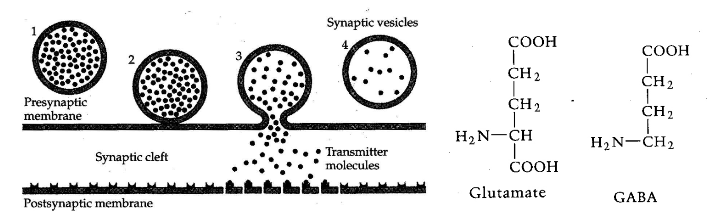
\includegraphics[width=0.9\textwidth]{Synaptic_cleft_project}
 \caption{Left: Illustration of the release of vesicle from an axon. The neurotransmitters (two chemical structures are shown to the right) travel diffusively across the synaptic cleft and are absorbed in the postsynaptic membrane at a distance $d$ away from the release point. The figure is taken from the project description \cite{Komp3150}, but originates from Thompson: "The Brain", Worth Publ., 2000.}
\label{fig:Synaptic_cleft}
\end{figure}

The solutions will be studied by implementation of three direct solver schemes and Monte Carlo based methods. For the direct solvers we will look in some detail at the Forward Euler scheme, the Backward Euler scheme and the Crank-Nicholson scheme for partial differential equations (PDEs). The methods are compared in terms of precision (i.e. local truncation errors) and stability. We also simulate the system as a random walk, first with a constant step length and equal probability of moving left and right. In the second approach we draw step lengths from a normal distribution. 

\section{Theory}
In this section we derive the analytical solution to the diffusion problem outlined above. The closed form expression of the solution, although it will take the form of an infinite sum, will be valuable in terms of judging the numerical results later. We also provide some background material on random walks and the link to diffusion. This is the basics of the Monte Carlo methods discussed in the method/algorithm section.

\subsection{Analytical solution}
To solve the one dimensional diffusion equation, 

\begin{equation}
\frac{\partial u}{\partial t} = \frac{\partial^2 u}{\partial x^2},
\label{eq:Basic_problem}
\end{equation}

with the boundary conditions in (\ref{eq:Boundary_condition}) and initial conditions in (\ref{eq:Initial_conditions}), we apply the standard \emph{separation of variables} ansatz:

\begin{equation}
 u(x,t) = v(x,t) + u_s(x) = X(x)T(t) + u_s(x)
\label{eq:Separation of variables}
\end{equation}

We here added the steady-state solution $u_s(x) = 1-x$ (this is just a particular solution of the differential equation which then forces $v(x,t)$ to obey Dirichlet boundary 
conditions), which trivially satisfies equation (\ref{eq:Basic_problem}). Inserting (\ref{eq:Separation of variables}) into equation (\ref{eq:Basic_problem})
and dividing by $XT$ yields:

\begin{equation}
\frac{1}{X} \frac{d^2 X}{dx} = \frac{1}{T}\frac{dT}{dt} = -k^2
\label{eq:Separated_equation}
\end{equation}

The last equality, i.e. both sides equal to a constant, follows since the left hand side is independent of $t$ and the right hand side independent of $x$. 
Looking first at the $X(x)$ equation, we realize that it is simply the harmonic oscillator equation with solution $X(x) = a\cos(kx) + b\sin(kx)$. 
Since we must have $X(0) = X(1) = 0$ after adding the steady-state solution, the boundary condition (\ref{eq:Boundary_condition}) translates to
$a = 0$ and  $\sin(k) = 0 \Rightarrow k_n = n\pi$ for $n \in \mathbb{N}$. We thus have:

\begin{equation}
X_n(x) = b_n \sin(n\pi)
\label{eq:Separated_X_solution}
\end{equation}

The equation for $T(t)$ is a separable first order differential equation and have solutions:

\begin{equation}
T_n(x) = \exp(-(n\pi)^2t)
\label{eq:Separated_T_solution}
\end{equation}

The general solution is then a sum of (possibly all) the modes $X_n(x)T_n(t)$:

\begin{equation}
u(x,t) = 1-x +\sum_{n=1}^{\infty} b_n \sin(n\pi x) e^{-(n\pi)^2t}
\label{eq:General_solution}
\end{equation}

The final step is to determine the coefficients $b_n$ such that $u(x,0)$ fits the initial conditions in equation (\ref{eq:Initial_conditions}). This can be rewritten as 

\begin{equation}
\sum_{n=1}^{\infty} b_n \sin(n\pi x) = v_0(x) =  \begin{cases} 0 & \mathrm{if} \hspace{2mm} x = 0 \\
x-1 & \mathrm{if} \hspace{2mm} x \in (0,1] \end{cases}
\label{eq:Initial_cond_fit}
\end{equation}

This rightmost expression is the initial condition for the solution $v(x,t)$ which will be discussed in the context of Monte Carlo methods later. The sum above is just the Fourier series of the odd extension of the function $v_0(x)$ on the interval $[0,1]$. The coefficients are determined by Fourier's trick (see for instance \cite{Boas}):

\begin{equation}
b_n = \frac{2}{L}\int_0^L dx \hspace{1mm} v_0(x)\sin\left( \frac{n \pi x}{L}\right) = 2\int_0^1 dx \hspace{1mm} (x-1) \sin(n\pi x) = -\frac{2}{n\pi}
\label{eq:Fourier_trick}
\end{equation}

We hence have arrived at the final closed form solution:

\begin{equation}
\boxed{u(x,t) = 1-x - \frac{2}{\pi} \sum_{n=1}^{\infty} \frac{\sin(n\pi x)}{n} e^{-(n\pi)^2t}}
\label{eq:Final_solution}
\end{equation}

\subsection{Random walks and diffusion}
\label{sec:RW}
We devote this section to studying how random walks in one dimension are linked to diffusion through the \emph{central limit theorem} when the number of steps become large. Much of the material in this section is based on \cite{Komp4130}. \\ 

Consider a random walk with $N$ steps of step length $\ell_0$ and no boundaries. Denote the probability of taking a step to the right by $p$ and to the left by $q = 1-p$
(a symmetric walk has of course $p=q=1/2$). One can quite easily be convinced that out of a total of $N$ steps, the probability that the walker has taken exactly $R$ steps 
to the right (and $L$ to the left, $R+L = N$) is given by the \emph{Bernoulli distribution}:

\begin{equation}
P_N(R) = \binom{N}{R} p^R q^{N-R}
\label{eq:RW_Bernoulli}
\end{equation}

The normalization, $\sum_{R=0}^N P_N(R) = 1$, follows readily from the binomial formula. By some small tricks with the binomial coefficients, one can use this distribution to find for instance $\langle R \rangle = Np$ and $\langle R^2 \rangle = (Np)^2 + Npq$. These quantities can in turn be exploited further to find the average displacement, 

\begin{equation}
\langle S \rangle = (2 \langle R \rangle - N)\ell_0 = N(p-q)\ell_0
\label{eq:RW_displacement}
\end{equation}

and square displacement:

\begin{equation}
\langle S^2 \rangle = (4\langle R^2 \rangle -4N\langle R \rangle +  N^2)\ell_0^2 = N^2(p-q)^2\ell_0^2 + 4Npq\ell_0^2
\label{eq:RW_displacement_sq}
\end{equation}

This yields the variance of the $N$-step walk:

\begin{equation}
\sigma_N^2 = \langle S^2 \rangle - \langle S \rangle^2 = 4Npq\ell_0^2 \propto N
\label{eq:RW_variance}
\end{equation}

The proportionality, meaning a distribution that widens proportional to the square root of time (time meaning the number of steps), is in fact a clear sign of a diffusion like process. We now move swiftly over to the large $N$ limit. The symmetric distribution ($p=q=1/2$) can be expanded using Stirling's formula, $N! \approx \sqrt{2\pi N} N^N e^{-N}$. Keeping only the lowest order in $S/(N\ell_0)$ gives the following result after some algebraic manipulations:

\begin{equation}
P_N(S) = \left( \frac{1}{2} \right)^N \frac{N!}{L!R!} \approx \sqrt{\frac{2}{\pi N}} e^{-S^2/(2N\ell_0^2)} \to \frac{1}{\sqrt{4\pi D t}} e^{-\frac{x^2}{4Dt}} = P(x,t)
\label{eq:RW_symmetric_largeN}
\end{equation}

The last expression is a properly normalized ($\int_{-\infty}^{\infty} dx \hspace{1mm} P(x,t) =1 $) continuum limit of the same distribution with some conventional choice of 
constants and $N$ basically replaced by time\footnote{The limit formally occurs by the replacements: $x = S$, $t = N\tau$ with $\tau$ the time of one step and 
$D = \ell_0^2/(2\tau)$ as diffusion constant. Normalization gives the correct prefactor.}. This continuum distribution is in fact more generally a consequence of 
\emph{the central limit theorem}. Briefly summarized, this theorem states that if variable $X = \sum_{i=1}^N x_i$ is the sum of some stochastically independent 
variables $x_i$ drawn from a distribution $p(x)$ with zero mean $\langle x \rangle = 0$ and finite variance $\sigma_x^2 \in \mathbb{R}^+$, the distribution $P(X)$ 
will tend to a Gaussian with variance $\sigma_X^2 = N\sigma_x^2$ as $N$ becomes large. \\

For free particles described by the concentration
$C(x,t) = NP(x,t)$ with $P(x,t)$ given as in equation (\ref{eq:RW_symmetric_largeN})\footnote{Observe also that $\lim_{t\to 0}C(x,t) = N\delta(x)$ – all particles located at $x=0$ initially.}, one can actually derive the diffusion equation by the use of Fick's law. 
Fick's law in one dimension for the distribution $P(x,t)$ states that the particle current is given by 

\begin{equation}
J_x = \frac{d}{dt} \int_x^{\infty} dx \hspace{1mm} C(x,t) = -D \frac{\partial C(x,t)}{\partial x},
\label{eq:Fick_law}
\end{equation}

for non-interacting particles.
This can be proven by direct differentiation. In higher dimensions, the law would more generally take the form 
$\boldsymbol{J}(\boldsymbol{r},t) = - D \nabla C(\boldsymbol{r},t)$. We now combine this law with the divergence theorem to show that the concentration leads to the diffusion equation. The starting point is the continuity equation, stating that the change of particles in the volume $V$ is equal to the particle flux out of the closed boundary $S$ of $V$:

\begin{align}
 \frac{d}{dt} \int_V dV \hspace{1mm} C(\boldsymbol{r},t) + \oint_S d\boldsymbol{S} \cdot \boldsymbol{J}(\boldsymbol{r},t) &=0 \Rightarrow \\
 \int_V dV \hspace{1mm} \frac{\partial C(\boldsymbol{r},t)}{\partial t} -D\oint_S d\boldsymbol{S} \cdot \nabla C(\boldsymbol{r},t) &=0 \Rightarrow \\
  \int_V dV \hspace{1mm} \frac{\partial C(\boldsymbol{r},t)}{\partial t}  -D\int_V dV \hspace{1mm} \nabla^2 C(\boldsymbol{r},t) &=0
\end{align}
This must hold for an arbitrarily chosen volume, and thus
\begin{equation}
\frac{\partial C(\boldsymbol{r},t)}{\partial t} - D \nabla^2 C(\boldsymbol{r},t) = 0
\label{eq:Diffusion_Gauss_theorem}
\end{equation}

This provides us with a basic understanding of the link between macroscopic phenomenon of diffusion  and 
a set of  discrete random walks that are easily simulated computationally. We will exploit this link when discussing Monte Carlo methods.


\subsection{Stability of matrix iterations}
\label{sec:Stability}
We here very briefly state a theorem (brought from \cite{Komp3150}) that will be applied in the discussion of the three direct solvers in the next section. \\

Suppose we are given the iteration $\boldsymbol{V}_i = A \boldsymbol{V}_{i-1}$ for some non-singular matrix $A$ and vectors $\boldsymbol{V}_i$. This implies that the vector after $n$ iterations is given in terms of the initial one as: $\boldsymbol{V}_n = A^n \boldsymbol{V}_0$. By expanding $\boldsymbol{V}_0$ in the eigenvector basis of $A$, we can quickly understand the following theorem quite intuitively: \\

\begin{theorem}
The solution to the iteration $\boldsymbol{V}_i = A \boldsymbol{V}_{i-1}$ will converge to a definite value if $\rho(A) < 1$, where $\rho(A)$ is the spectral radius of $A$:

\begin{equation}
\rho(A) = \mathrm{max}\{\lvert \lambda_n \rvert : \mathrm{det}(A-\lambda_n\id)=0 \}
\label{eq:Spectral_radius}
\end{equation}
\end{theorem}

This is a central concept in Chaos theory when determining for example the stability of flows and maps\footnote{This is for instance covered in Predrag Cvitanović's book on chaos theory: http://chaosbook.org/.}.

\section{Method / Algorithm}
This section is devoted to the discussion of the three deterministic schemes for PDEs mentioned earlier. We derive the algorithms and investigate their stability properties expressed in terms of $\Delta x$ and $\Delta t$. First some general nomenclature. We discretize the interval $[0,1]$ with a step length determined by some integer $n$: 

\begin{equation}
 \Delta x = \frac{1}{n+1}
\label{eq:Step_length}
\end{equation}

such that $x \mapsto x_i = i\Delta x$ for $i \in \{0,1,\dots,n+1 \}$. The boundary conditions fixes the values at $i=0$ and $i=n+1$, so we are left with $n-1$ internal points
of interest. A corresponding discretization in time is given by $\Delta t$ (we will later discuss how this should be chosen in terms of $\Delta x$, i.e. $n$).
This means that $t\mapsto t_j = j\Delta t$ for $j\in \mathbb{N}$. The following discussion will be made in the context of the diffusion equation, here written compactly
as $u_{xx} = u_t$ with the subscripts referring to derivatives. After discretization we use the notation $u(x,t) \mapsto u(x_i, t_j) \equiv u_{i,j}$. The following definition 
will also appear frequently in what follows:

\begin{equation}
 \alpha \equiv \frac{\Delta t}{\Delta x^2}
\label{eq:Step_parameter}
\end{equation}

Much the following discussion is closely related to the lecture notes \cite{Komp3150}. We try to establish a notation similar to the implementation found in the written code. We note that the Forward Euler method was implemented to find $u(x,t)$ directly while the two implicit schemes and the Monte Carlo methods were written to solve for $v(x,t)$ (adding $u_s(x) = 1-x$ in the end) due to its more easily handled Dirichlet boundary conditions. \\

In the last subsection we discuss the two Monte Carlo based algorithms for a random walk that were implemented during the work with this project. We also discuss the basic terms related to Monte Carlo samplings that are relevant in this context.

\subsection{Forward Euler scheme}
In this scheme we use the two simplest possible approximations for the derivatives $u_{xx}$ and $u_t$:

\begin{equation}
u_{xx} \approx \frac{u(x+\Delta x,t)-2u(x,t)+u(x-\Delta x, t)}{\Delta x^2} \mapsto \frac{1}{\Delta x^2} (u_{i+1,j}-2u_{i,j}+u_{i-1,j})
\label{eq:Forward_uxx}
\end{equation}

and the asymmetric (forward) time derivative

\begin{equation}
u_{t} \approx \frac{u(x,t+\Delta t)-u(x, t)}{\Delta t} \mapsto \frac{1}{\Delta t} (u_{i,j+1}-u_{i,j})
\label{eq:Forward_ut}
\end{equation}

This leads directly to an explicit scheme when equating the above expressions:

\begin{align}
u_{xx} &= u_t \Rightarrow \\
 \frac{1}{\Delta x^2} (u_{i+1,j}-2u_{i,j}+u_{i-1,j}) &= \frac{1}{\Delta t} (u_{i,j+1}-u_{i,j}) \Rightarrow \\
 u_{i,j+1} &= \alpha u_{i+1,j} + (1-2\alpha)u_{i,j} + \alpha u_{i-1,j}
\label{eq:Forward_Euler_scheme}
\end{align}

\begin{figure}[h!tb]
 \centering
 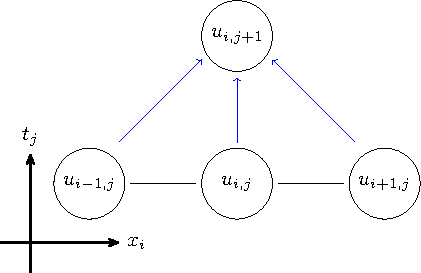
\includegraphics[width=0.4\textwidth]{Grid_FE-figure0}
 \caption{Forward Euler scheme stencil for the $(1+1)$-dimensional diffusion equation. $u_{i,j}$ is the discretized solution at position $x_i$ and time $t_j$.}
 \label{fig:FE_grid}
\end{figure}

This scheme is explicit in the sense that it gives a recipe of how to find the solution at the next time step given the solution at the previous one. It should be initialized with the initial condition, $u_{i,0} = u_0(x_i)$ as given in equation (\ref{eq:Initial_conditions}). In terms of a matrix equation we can write:

\begin{align}
\boldsymbol{U}_{j+1} &= A \boldsymbol{U}_j + \boldsymbol{U}_{boundary}\\
\begin{bmatrix}
u_{1,j+1} \\ u_{2,j+1} \\ \vdots \\ u_{n-1,j+1}
\end{bmatrix}
&=
\begin{bmatrix}
 1-2\alpha & \alpha & 0 & \cdots & 0 & 0 \\
 \alpha & 1-2\alpha & \alpha & \cdots & 0 & 0 \\
 \vdots & \vdots & \vdots & \ddots & \vdots & \vdots \\
 0 & 0 & 0 & \cdots & \alpha & 1-2\alpha \\
\end{bmatrix}
\begin{bmatrix}
u_{1,j} \\ u_{2,j} \\ \vdots \\ u_{n-1,j}
\end{bmatrix}
+
\begin{bmatrix}
\alpha \\ 0 \\ \vdots \\ 0
\end{bmatrix}
\label{eq:Forward_Euler_matrix}
\end{align}

where we explicitly took care of the boundary conditions in the constant vector being added (since $u_{0,j} = 1$ and $u_{n,j} = 0$) and only care about the $n-1$ internal points. It is appropriate, also for later reference, to decompose the matrix as $A = \id - \alpha B$ where the elements of $B$ can be expressed in terms of Kronecker deltas: 

\begin{equation}
B_{i,j} = 2\delta_{i,j}-\delta_{i+1,j}-\delta_{i-1,j}
\label{eq:Matrix_B}
\end{equation}

The subscripts here refer to matrix indices and have nothing to do with time and space coordinates as earlier. \\

\textbf{Algorithm} \newline
The implementation of the explicit scheme is rather straight forward (basically equation (\ref{eq:Forward_Euler_scheme})). We have shown the core of the function \texttt{Forward\_Euler()} in listing \ref{lst:FE}. The function \texttt{Output\_write()} is a function that writes the results of a given time step – more precisely at \texttt{iter1} and \texttt{iter2} corresponding to absolute times $t_1 = 0.05$ and $t_2 = 0.3$ – to a plain text file for later plotting. The function \texttt{func(double x)} is a function that reflects the (trivial) initial conditions of $u$: $u(x,0)$.

\lstset{language=C++,caption={Code sample: the main content of the function \texttt{void Forward\_Euler()}. Its full implementation can be found in \texttt{Project5\_d.cpp}.},label={lst:FE}}
\begin{center}
\begin{lstlisting}
  u(0) = unew(0) = 1.0;
  u(n) = unew(n) = 0.0;
  // Initialize the vector acording to the initial condition in func(x):
  for (int i=1; i < n; i++) { // Initialize only interior solution
  	x_val = i*delta_x;
  	u(i) = func(x_val);
  	unew(i) = 0;
  }
  // Time integration according to the explicit scheme:
  for (int j = 1; j <= tsteps; j++) {
  	t_val = j*delta_t;
  	for (int i = 1; i < n; i++) {
  		unew(i) = alpha*u(i-1) + (1 - 2*alpha)*u(i) + alpha*u(i+1);
  	}
  	u = unew;
  	if (j == iter1 or j == iter2) {
  	  // Write current values (all x) to txt file:
  	  Output_write(unew, t_val, n);
    }
  }
\end{lstlisting}
\end{center}

\textbf{Truncation errors} \newline
The discretized equations in (\ref{eq:Forward_uxx}) and (\ref{eq:Forward_ut}) are easily seen to come from the Taylor expansions (with step lengths $\Delta x$ and $\Delta t$ respectively) around $u(x,t)$:

\begin{align}
u(x\pm\Delta x,t) &= u(x,t) \pm \frac{\partial u(x,t)}{\partial x}\Delta x + \frac{1}{2}\frac{\partial^2 u(x,t)}{\partial x^2}\Delta x^2 \pm \frac{1}{6}\frac{\partial^3 u(x,t)}{\partial x^3}\Delta x^3 +  \mathcal{O}(\Delta x^4)
\label{eq:Forward_Euler_expansions1} \\
u(x,t\pm \Delta t) &= u(x,t) \pm \frac{\partial u(x,t)}{\partial t}\Delta t + \mathcal{O}(\Delta t^2)
\label{eq:Forward_Euler_expansions2}
\end{align}

and readily spell out for us that the Forward Euler scheme gives rise to errors of orders $\mathcal{O}(\Delta t)$ and $\mathcal{O}(\Delta x^2)$ when inserted into (\ref{eq:Forward_uxx}) and (\ref{eq:Forward_ut}). These errors are local approximation errors. \\

% SHOULD THESE BE FOUND EXACT?

\textbf{Stability condition} \newline
To determine for what combinations of $\Delta t$ and $\Delta x$ the Forward Euler scheme is stable, we investigate the spectral radius – according to section \ref{sec:Stability} – of the matrix $B$ (the other part of $A = \id - \alpha B$ is simply $\id$ and gives rise to a unit contribution to the eigenvalues):

\begin{align}
(B\boldsymbol{v})_i &= \lambda_i v_i \\
\sum_{j=1}^n [2\delta_{i,j}-\delta_{i+1,j}-\delta_{i-1,j}]v_j &= \lambda_i v_i
\label{eq:Forward_Euler_stability1}
\end{align}

We continue with expanding the vector components in a sine basis $v_i = \sin(i\theta)$ with $\theta = \pi/(n+1)$ such that

\begin{align}
\sum_{j=1}^n [2\delta_{i,j}-\delta_{i+1,j}-\delta_{i-1,j}]v_j &= \lambda_i v_i \\
2 \sin(i\theta) - \sin\left((i+1)\theta\right) - \sin\left((i-1)\theta\right) &= \lambda_i \sin(i\theta) \\
2(1-\cos(\theta)) &= \lambda_i
\label{eq:Forward_Euler_stability2}
\end{align}

Hence in order to have $\rho(A) < 1$, we must have

\begin{equation}
\lvert 1-2\alpha(1-\cos(\theta)) \rvert < 1 \Rightarrow \alpha = \frac{\Delta t}{\Delta x^2} \leq \frac{1}{2}
\label{eq:Forward_Euler_stability3}
\end{equation}

The extremal eigenvalue formally occurs when $\theta = \pi$ (a value which is never reached for $i \in \{1,\dots, n\}$) and the final inequality follows.

\subsection{Backward Euler scheme}
The Backward Euler scheme (just like for ordinary differential equations) exploits a time derivative approximation with a function evaluation \emph{backwards} in time and the same approximation for $u_{xx}$ as in equation (\ref{eq:Forward_uxx}). We (re)state both approximations to have a clear argument:

\begin{equation}
u_{xx} \approx \frac{u(x+\Delta x,t)-2u(x,t)+u(x-\Delta x, t)}{\Delta x^2} \mapsto \frac{1}{\Delta x^2} (u_{i+1,j}-2u_{i,j}+u_{i-1,j})
\label{eq:Backward_uxx}
\end{equation}

\begin{equation}
u_{t} \approx \frac{u(x,t)-u(x,t-\Delta t)}{\Delta t} \mapsto \frac{1}{\Delta t} (u_{i,j}-u_{i,j-1})
\label{eq:Backward_ut}
\end{equation}

Equating these leaves us with:

\begin{align}
u_{xx} &= u_t \Rightarrow \\
 \frac{1}{\Delta x^2} (u_{i+1,j}-2u_{i,j}+u_{i-1,j}) &= \frac{1}{\Delta t} (u_{i,j}-u_{i,j-1}) \Rightarrow \\
 u_{i,j-1} &= -\alpha u_{i+1,j} + (1+2\alpha)u_{i,j} - \alpha u_{i-1,j}
\label{eq:Backward_Euler_scheme}
\end{align}

\begin{figure}[h!tb]
 \centering
 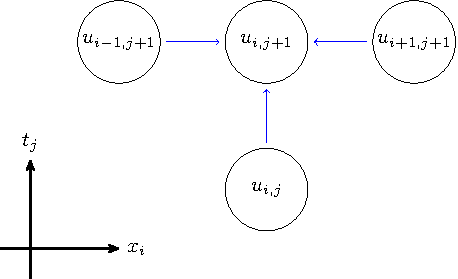
\includegraphics[width=0.4\textwidth]{Grid_BE-figure0}
 \caption{Backward Euler scheme stencil for the $(1+1)$-dimensional diffusion equation. $u_{i,j}$ is the discretized solution at position $x_i$ and time $t_j$.}
 \label{fig:BE_grid}
\end{figure}

This recursion relation backwards in time does, as compared to the Forward Euler scheme, not give us the solution for the next time step in terms of the previous one explicitly. 
At this point we switch to solving for $v(x,t) \mapsto v_{i,j}$ instead of $u(x,t)$ to more easily control the boundary conditions. Note that the initial condition for $v(x,t)$ is given in (\ref{eq:Initial_cond_fit}). This time the matrix equations takes the following form:

\begin{align}
C \boldsymbol{V}_j &= \boldsymbol{V}_{j-1} \\
\begin{bmatrix}
 1+2\alpha & -\alpha & 0 & \cdots & 0 & 0 \\
 -\alpha & 1+2\alpha & -\alpha & \cdots & 0 & 0 \\
 \vdots & \vdots & \vdots & \ddots & \vdots & \vdots \\
 0 & 0 & 0 & \cdots & -\alpha & 1+2\alpha \\
\end{bmatrix}
\begin{bmatrix}
v_{1,j} \\ v_{2,j} \\ \vdots \\ v_{n-1,j}
\end{bmatrix}
&=
\begin{bmatrix}
v_{1,j-1} \\ v_{2,j-1} \\ \vdots \\ v_{n-1,j-1}
\end{bmatrix}
\label{eq:Backwards_Euler_matrix}
\end{align}

with $C = \id + \alpha B$ and $B$ is the same as in (\ref{eq:Matrix_B}). This asks for, at each time step $j$, nothing else than a set of linear equations to be solved. Phrased differently, a matrix inversion (meaning we must find $C^{-1}$ with $C$ tridiagonal as above) would give us the solution at each time step straight away: $\boldsymbol{V}_j = C^{-1} \boldsymbol{V}_{j-1}$. However, a matrix-vector multiplication at each time step is computationally consuming as it costs $\mathcal{O}(n^2)$ FLOPS and the matrix inversion even worse with its $\mathcal{O}(n^3)$ FLOPS. From Project 1, however, we know that solving such equations for a tridiagonal matrix can be done by an algorithm that takes only $\mathcal{O}(n)$ FLOPS\footnote{In project 1 we used an algorithm requiring $8(n-1)$ FLOPS for solving a tridiagonal set of linear equations.}; far superior when the dimension becomes large. \\

\textbf{Algorithm} \newline
To use the Backward Euler scheme we chose to bring in the tridiagonal matrix solver from project 1. It is gathered in a function called \texttt{void tridiag()} which makes use of armadillo vectors. The basic implementation of the implicit scheme (meaning equation (\ref{eq:Backwards_Euler_matrix})) is shown in listing \ref{lst:BE}. This time, \texttt{func2(double x)} is a function which returns the initial condition for $v$, not $u$ (given in equation (\ref{eq:Initial_cond_fit})).

\lstset{language=C++,caption={Code sample: the main content of the function \texttt{void Backward\_Euler()}. Its full implementation can be found in \texttt{Project5\_d.cpp}.},label={lst:BE}}
\begin{center}
\begin{lstlisting}
  // Boundary conditions:
  v(0) = vnew(0) = 0.0;
  v(n) = vnew(n) = 0.0;
  a = c = -alpha; 
  b = 1+2*alpha; 
  // Initialize the vector according to the initial condition in func2(x):
  for (int i=1; i < n; i++) { // Initialize only interior solution
    x_val = i*delta_x; v(i) = func2(x_val); vnew(i) = 0;
  }
  // Time loop:
  for (int j = 1; j <= tsteps; j++) {
    t_val = j*delta_t;
    tridiag(a, b, c, v, vnew, n-1); // Solver for tridiagonal matrix problem
    v(0) = vnew(0) = 0.0;
    v(n) = vnew(n) = 0.0;
    // Update old result for next loop iteration:
    v = vnew;
    if (j == iter1 or j == iter2) {
      for (int l=1; l<n; l++) {
        v_val = vnew(l);
        unew(l) = v_val + 1.0 - l*delta_x;
      }
      unew(0) = 1.0; unew(n) = 0.0;
      // Write current values (all x) to txt file:
      Output_write(unew, t_val, n);
    }
  }
\end{lstlisting}
\end{center}

\textbf{Truncation errors} \newline
Equations in (\ref{eq:Backward_uxx}) and (\ref{eq:Backward_ut}), just as for the Forward Euler scheme, stem from the Taylor expansions (with step lengths $\Delta x$ and $\Delta t$ respectively) as in equation (\ref{eq:Forward_Euler_expansions1}) and (\ref{eq:Forward_Euler_expansions2}). It is straight forwardly seen that this scheme gives identical truncation errors – of orders $\mathcal{O}(\Delta t)$ and $\mathcal{O}(\Delta x^2)$ – just as in the explicit method. These are again local approximation errors. \\

\textbf{Stability condition} \newline
This time we need to consider the spectral radius of $C^{-1} = (\id + \alpha B)^{-1}$. However, the work done in the stability discussion of the Forward Euler method gives us the answer quickly. We know from the earlier discussion that the eigenvalues of $C$ are strictly positive and larger than unity: $\mu_i = 1 + 2\alpha(1-\cos(\theta)) > 1$. This implies that the eigenvalues of $C^{-1}$ are strictly less than unity\footnote{We can understand this result from the following small argument. Assume the eigenvalue equation $A\boldsymbol{x} = \lambda \boldsymbol{x}$. Applying $A^{-1}$ to both sides and rearranging implies that $A^{-1}\boldsymbol{x} = \frac{1}{\lambda} \boldsymbol{x}$. This means that if $\lambda$ is an eigenvalue of $A$, then $\lambda^{-1}$ is an eigenvalue of $A^{-1}$.}: $\mu_i^{-1} < 1$. Furthermore we have $\rho(C^{-1}) < 1$ for all combinations of $\Delta t$ and $\Delta x$; a rather weak stability condition (i.e. no restrictions on the step lengths). Thus the (small) increase in FLOPS when using the implicit scheme in favour of the explicit scheme, does pay off in a much weaker stability condition.

\subsection{Crank-Nicolson scheme}
The Crank-Nicolson scheme is, in a sense, an equally weighted compromise between the forward Euler scheme and the backward Euler scheme. To see this explicitly, let us rephrase and compare the two previous schemes:

\begin{equation}
 \frac{1}{\Delta t} (u_{i,j}-u_{i,j-1}) = \frac{1}{\Delta x^2} (u_{i+1,j-1}-2u_{i,j-1}+u_{i-1,j-1}) \hspace{10pt} \mathrm{(Forward \hspace{2mm} Euler)}
\end{equation}

\begin{equation}
 \frac{1}{\Delta t} (u_{i,j}-u_{i,j-1}) = \frac{1}{\Delta x^2} (u_{i+1,j}-2u_{i,j}+u_{i-1,j}) \hspace{10pt} \mathrm{(Backward \hspace{2mm} Euler)}
\end{equation}

Adding the two equations gives the Crank-Nicolson scheme\footnote{A more general approach would be to assign different weights the two contributions in what is known as a $\theta$-rule \cite{Komp3150}.}:

\begin{align}
\frac{2}{\Delta t} (u_{i,j}-u_{i,j-1}) &= \frac{1}{\Delta x^2} (u_{i+1,j}-2u_{i,j}+u_{i-1,j}+u_{i+1,j}-2u_{i,j}+u_{i-1,j} ) \Rightarrow \\
 -\alpha u_{i+1,j} + 2(1+\alpha)u_{i,j} -\alpha u_{i-1,j} &= \alpha u_{i+1,j-1} + 2(1-\alpha) u_{i,j-1} + \alpha u_{i-1,j-1}
\label{eq:Crank_Nicoloson_scheme}
\end{align}

\begin{figure}[h!tb]
 \centering
 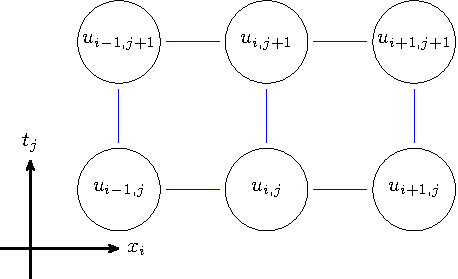
\includegraphics[width=0.4\textwidth]{Grid_CN-figure0}
 \caption{Crank-Nicolson scheme stencil for the $(1+1)$-dimensional diffusion equation. $u_{i,j}$ is the discretized solution at position $x_i$ and time $t_j$.}
 \label{fig:CN_grid}
\end{figure}

or in matrix notation (we also this time consider $v(x,t)$ instead of $u(x,t)$ due to the simple boundary conditions):

\begin{align}
(2\id + \alpha B) \boldsymbol{V}_j &= (2\id - \alpha B) \boldsymbol{V}_{j-1} \\
\begin{bmatrix}
 2+2\alpha & -\alpha & 0 & \cdots & 0 & 0 \\
 -\alpha & 2+2\alpha & -\alpha & \cdots & 0 & 0 \\
 \vdots & \vdots & \vdots & \ddots & \vdots & \vdots \\
 0 & 0 & 0 & \cdots & -\alpha & 2+2\alpha \\
\end{bmatrix}
\begin{bmatrix}
v_{1,j} \\ v_{2,j} \\ \vdots \\ v_{n-1,j}
\end{bmatrix}
&= \\
\begin{bmatrix}
 2-2\alpha & \alpha & 0 & \cdots & 0 & 0 \\
 \alpha & 2-2\alpha & \alpha & \cdots & 0 & 0 \\
 \vdots & \vdots & \vdots & \ddots & \vdots & \vdots \\
 0 & 0 & 0 & \cdots & \alpha & 2-2\alpha \\
\end{bmatrix}
&\begin{bmatrix}
v_{1,j-1} \\ v_{2,j-1} \\ \vdots \\ v_{n-1,j-1}
\end{bmatrix}
\label{eq:Crank_Nicolson_matrix}
\end{align}

Thus $\boldsymbol{V}_j = (2\id+\alpha B)^{-1}(2\id - \alpha B)\boldsymbol{V}_{j-1}$. This looks very similar to the Backward Euler scheme, the only difference being that we must 
at each time step first calculate $\tilde{\boldsymbol{V}}_{j-1} = (2\id - \alpha B)\boldsymbol{V}_{j-1}$ before sending $(2\id + \alpha B)\boldsymbol{V}_j = \tilde{\boldsymbol{V}}_{j-1}$ to the tridiagonal matrix solver. \\

\textbf{Algorithm} \newline
The Crank-Nicolson scheme makes use of the same tridiagonal matrix solver as the implicit scheme. The main difference from the previous scheme is however that we must add the calculation of $\tilde{\mathbf{V}}_{j-1}$ before passing the problem on to \texttt{tridiag()}. The main content of the written Crank-Nicolson function is shown in listing \ref{lst:CN}. 

\lstset{language=C++,caption={Code sample: the main content of the function \texttt{void Crank\_Nicolson()}. Its full implementation can be found in \texttt{Project5\_d.cpp}.},label={lst:CN}}
\begin{center}
\begin{lstlisting}
// Boundary conditions:
  v(0) = vnew(0) = 0.0;
  v(n) = vnew(n) = 0.0;
  a = c = -alpha; 
  b = 2+2*alpha; 
  for (int i=1; i < n; i++) { // Initialize only interior solution
    x_val = i*delta_x; v(i) = func2(x_val); vnew(i) = 0;
  }
  // Time loop: 
  for (int j = 1; j <= tsteps; j++) {
    t_val = j*delta_t;
    for (int l=1; l < n; l++) {
         y(l) = alpha*v(l+1) + (2 - 2*alpha)*v(l) + alpha*v(l-1);
    }
    tridiag(a, b, c, y, vnew, n-1); // Solver for tridiagonal matrix goes here.
    v(0) = vnew(0) = 0.0;
    v(n) = vnew(n) = 0.0;
    // Update old result for next loop iteration:
    v = vnew;
    if (j == iter1 or j == iter2) {
      for (int l=1; l<n; l++) {
        v_val = vnew(l);
        unew(l) = v_val + 1.0 - l*delta_x;
      }
      unew(0) = 1.0; unew(n) = 0.0;
      // Write current values (all x) to txt file:
      Output_write(unew, t_val, n);
    }
  }
\end{lstlisting}
\end{center}

\textbf{Truncation errors} \newline
The Crank-Nicolson scheme was presented above as the sum of two equally weighted contributions to $u_t$ – at steps $j+1$ and $j$ (figure \ref{fig:CN_grid}). 
The formulas for $u_{xx}$ were not altered, so the truncation errors in $x$ are still of the same order $\mathcal{O}(\Delta x^2)$. To see what happens to the truncation 
in $t$, we can Taylor expand the involved quantities around $t' = t + \Delta t /2$ and only study the errors in powers of $\Delta t$:

\begin{align}
u(x\pm\Delta x,t+\Delta t) &= u(x,t') \pm \frac{\partial u(x,t')}{\partial x}\Delta x + \frac{1}{2}\frac{\partial^2 u(x,t')}{\partial x^2}\Delta x^2  \nonumber \\
&+ \frac{\partial u(x,t')}{\partial t}\frac{\Delta t}{2} + \frac{1}{2}\frac{\partial^2 u(x,t')}{\partial t^2}\frac{\Delta t^2}{4} \pm \frac{\partial^2 u(x,t')}{\partial x \partial t}\frac{\Delta x \Delta t}{2} + \mathcal{O}(\Delta t^3)
\label{eq:Crank_Nicolson_expansions1} \\
u(x\pm\Delta x,t) &= u(x,t') \pm \frac{\partial u(x,t')}{\partial x}\Delta x + \frac{1}{2}\frac{\partial^2 u(x,t')}{\partial x^2}\Delta x^2 \nonumber \\
&- \frac{\partial u(x,t')}{\partial t}\frac{\Delta t}{2} + \frac{1}{2}\frac{\partial^2 u(x,t')}{\partial t^2}\frac{\Delta t^2}{4} \mp \frac{\partial^2 u(x,t')}{\partial x \partial t}\frac{\Delta x \Delta t}{2} + \mathcal{O}(\Delta t^3)
\label{eq:Crank_Nicolson_expansion2} \\
u(x,t+\Delta t) &= u(x,t') + \frac{\partial u(x,t')}{\partial t}\frac{\Delta t}{2} + \frac{1}{2}\frac{\partial^2 u(x,t')}{\partial t^2}\frac{\Delta t^2}{4}  + \mathcal{O}(\Delta t^3)
\label{eq:Crank_Nicolson_expansion3} \\
u(x,t) &= u(x,t') - \frac{\partial u(x,t')}{\partial t}\frac{\Delta t}{2} + \frac{1}{2}\frac{\partial^2 u(x,t')}{\partial t^2}\frac{\Delta t^2}{4}  + \mathcal{O}(\Delta t^3)
\label{eq:Crank_Nicolson_expansion4}
\end{align}

Putting these expansions carefully into equation (\ref{eq:Crank_Nicoloson_scheme}) (with the discretized labellings such as $u(x+\Delta x,t) = u_{i+1,j}$ etc.) and collecting the surviving terms, one can quite easily see that the terms to order $\mathcal{O}(\Delta t)$ cancel (this is in fact due to the equal weighting of the Forward and Backward Euler methods in the definition of the Crank-Nicolson scheme). The leading order truncation error in time is then seen to be $\mathcal{O}(\Delta t^2)$ – an improvement as compared to the Forward and Backward Euler schemes. But note once more that these are local errors. \\

\textbf{Stability condition} \newline
We need to look at the spectral radius of $(2\id + \alpha B)^{-1}(2\id -\alpha B)$. We can also this time reuse some earlier derived results. Recall the eigenvalues of 
$B$: $\lambda_i = 2(1-\cos(\theta) ) \in (0,4]$. Next, note that
\begin{align}
 (2\id+\alpha B)^{-1}B &= (2\id+\alpha B)^{-1}B(2\id+\alpha B)(2\id+\alpha B)^{-1}\nonumber\\
 &= (2\id+\alpha B)^{-1}(2\id+\alpha B)B(2\id+\alpha B)^{-1}\nonumber\\
 &= B(2\id+\alpha B)^{-1}
\end{align}
so that $(2\id+\alpha B)^{-1}$ and $(2\id+\alpha B)$ commute.
The spectral radius condition thus translates to the following in this case\footnote{
A theorem by Gelfand (1941) establishes a link between the spectral radius and the matrix norm $\norm{\cdot}$. It states that for any matrix norm $\norm{\cdot}$ we have 
$\rho(A) = \lim_{k\to \infty} \norm{A^k}^{1/k}$. From this it follows that \emph{commuting} matrices $A$ and $B$ satisfy (the matrix norm is submultiplicative): 
$\rho(AB) \leq \rho(A)\rho(B)$. We here emphasise that the  submultiplicativity of the spectral radius is not always present; it is a non-trivial property of matrices.}:
\begin{equation}
\rho\left( (2\id + \alpha B)^{-1}(2\id -\alpha B) \right) \leq \rho\left( (2\id + \alpha B)^{-1}\right)\rho\left((2\id -\alpha B) \right) < 1 \Rightarrow \frac{\lvert 2-\alpha \lambda_i\rvert}{\lvert 2+\alpha \lambda_i \rvert} < 1
\label{eq:Crank_Nicolson_spectralrad}
\end{equation}
This inequality is quite trivially seen to be satisfied since $\lambda_i > 0$. It is even more clearly seen by considering the two cases $\alpha\lambda_i < 2$ and $\alpha\lambda_i > 2$ separately. In total, we arrive at the same condition as for the Backward Euler scheme: all combinations of $\Delta t$ and $\Delta x$ results in a stable solution.

\subsection{Monte Carlo methods and random walks}
\label{sec:MC_method}
The basic background of the Monte Carlo approach to simulating diffusion is already outlined in section \ref{sec:RW}. In the approach of implementing this as a numerical
simulation, we follow Farnell and Gibson \cite{Farnell} to some extent. \\

Looking back at equation (\ref{eq:RW_symmetric_largeN}) and keeping in mind that we have put $D = 1$, we imagine that we simulate $N$ symmetric random walks with a step length 
$\ell_0$. This $\ell_0$ is now fixed by the choice of diffusion constant and time step $\Delta t$ since
$D = \ell_0^2/(2\Delta t) \Rightarrow \ell_0 = \sqrt{2D\Delta t} = \sqrt{2\Delta t}$. Another possibility that in the large $N$ limit should result in the same simulation,
is to use a varying step length, $\ell_0 = \sqrt{2\Delta t}\xi$ and $\xi$ drawn from a normal distribution with mean 0 and standard deviation 1. 
This time, the direction of the step is encoded in the sign of $\xi$ and the walk is still statistically symmetric. These are the two approaches we have implemented.\\

We chose to do the simulation with respect to $v(x,t)$ (adding $u_s(x)$ in the end) due to the absorbing boundary conditions  that $v(x,t)$ satisfies: $v(0,t) = v(1,t) = 0$. In terms of the simulation, this means that we simply check whether a particle hit the left or right boundary for
each step, and if it does, it is removed from the simulation still contributing to the number of cycles. Each non-absorbed walker must make $N_t$ steps where $N_t = t/\Delta t$ and $t$ is
the final time. \\

In addition, since the simulation is done for $v(x,t)$, with the initial condition $v(x,0) = x-1$ for $x\in (0,1)$, we draw the starting position of each walker from a PDF according to the initial distribution:

\begin{equation}
p(x) = 2(1-x)
\label{eq:MC_initial_dist}
\end{equation}

with the factor of 2 ensuring normalization $\int_0^1 dx \hspace{1mm} p(x) = 1$. Since we in practice draw numbers $r$ from a uniform distribution on the unit interval $r \in [0,1]$ (using \texttt{ran0()} from \cite{Komp3150}), we must perform a mapping that satisfies the differential equation $p(x)dx = dr$, yielding the solution:

\begin{equation}
r(x) = 2x-x^2 \hspace{10pt} \mathrm{and} \hspace{10pt} x(r) = 1 - \sqrt{1-r}
\label{eq:MC_prob_mapping}
\end{equation}

The final positions of each walker is stored in an array called \texttt{walk\_position[]}. This array is used to produce normalized histograms in python. In the code piece shown in listing \ref{lst:MC_uniform} (relevant for the constant step length simulation) we have added some more features. Firstly, we have restricted the initial position to be an integer multiple of $\ell_0$ (the allowed values are stored in \texttt{possible\_pos[]}) such that the final histogram bins can be deterministically chosen to fit the grid. This feature is removed when the step is drawn from a normal distribution. Secondly, we keep track of the number of the escaped particles (for later normalization) in the variable \texttt{N} and keep iterating until a total of \texttt{number\_walks} walkers have gotten a definite final position. This means that we in practice perform \texttt{number\_walks + N} walks – a number which intuitively will increase with the number of time steps as more and more walkers escape. \\

The variance of each walker, which is stored in \texttt{walk\_variance[]}, is averaged over all walkers and the corresponding standard deviation is in the end used  
as a measure of the statistical error $\sigma_t = \tilde{\sigma}/\sqrt{N_t}$ with $\tilde{\sigma}^2$ being the variance averaged over all walkers. The histograms are 
multiplied with at factor \texttt{0.5*number\_walks/(number\_walks + N)} to take into account the fact that \texttt{N} walkers escaped and the initial distribution had area 
of $1/2$. The histograms and the plots are all produced in the python scripts \texttt{Project5\_f.py}, \texttt{Project5\_g.py}, \texttt{Project5\_MCplotting1.py} and 
\texttt{Project5\_MCplotting2.py}. We finally note that the function which produces normally distributed step lengths was taken from the project description 
\cite{Komp3150} and is called \texttt{gaussian\_deviate()}.  \\

\lstset{language=C++,caption={Code sample: the main content of the Monte Carlo approach with random walks. The full implementations can be found in \texttt{Project5\_f.cpp} (constant step length) and \texttt{Project5\_g.cpp} (normal distributed step length).},label={lst:MC_uniform}}
\begin{center}
\begin{lstlisting}
// outer loop over walkers:
for (int trial=0; trial < number_walks; trial++){
    // inner loop over walkers:
    hit_wall = 1;
    // Checking whether the walker went outside or not:
    while (hit_wall == 1) {
      position = 0.0;
      dummy = 2.0; // Some random (and large) number to ensure new position is found
      r2 = ran0(&idum2);
      // Mapping to initial probability distribution:
      y = 1.0 - sqrt(1.0-r2);
      local_av2 = local_average = 0.0;
      // Finding closest multiple of l0:
      for (int j=1; j<n; j++) {
        val = fabs(possible_pos[j] - y);
        if (val < dummy) { dummy = val; position = possible_pos[j]; }
      }
      flag = 0;
      for (int tstep = 1; tstep <= tsteps; tstep++) {
        r = ran0(&idum);
        // Move right:
        if (r <= move_probability){
          if (1.0 - l0 - position <= eps){flag = 1; N += 1; break; } // Hit right wall: discard!
          else{ position += l0; }
        }
        // Move left:
        if (r > move_probability){
          if (position - l0 <= eps){ flag = 1; N += 1; break; } // Hit left wall: discard!
          else { position -= l0; }
        }
        local_average += position; local_av2 += position*position;
      }  // end of loop over walks
      if (flag == 0){ hit_wall = 0; } // Walk ended without hitting a wall!
    } // end of loop over trials

    local_average /= ((double) tsteps); local_av2 /= ((double) tsteps);
    walk_position[trial] = position;
    walk_variance[trial] = local_av2 - local_average*local_average;
}
\end{lstlisting}
\end{center}

\section{Results}
We provide a collection of plots and tables that summarize and compare the five different methods in terms of computation speed and accuracy. Figures \ref{fig:Three_methods10} and \ref{fig:Three_methods100} show the solutions found with the three direct solvers for $\Delta x = 1/10$ and $\Delta x = 1/100$ as spatial step length respectively. Figure \ref{fig:MC_uniform} shows the results of a simulation of the process as a random walk with constant step length and equal probability of moving left and right. In figure \ref{fig:MC_gaussian} the results of similar computations are shown, but with a step length drawn from a normal distribution.

\begin{figure}[h!tb]
 \centering
 \mbox{\subfigure{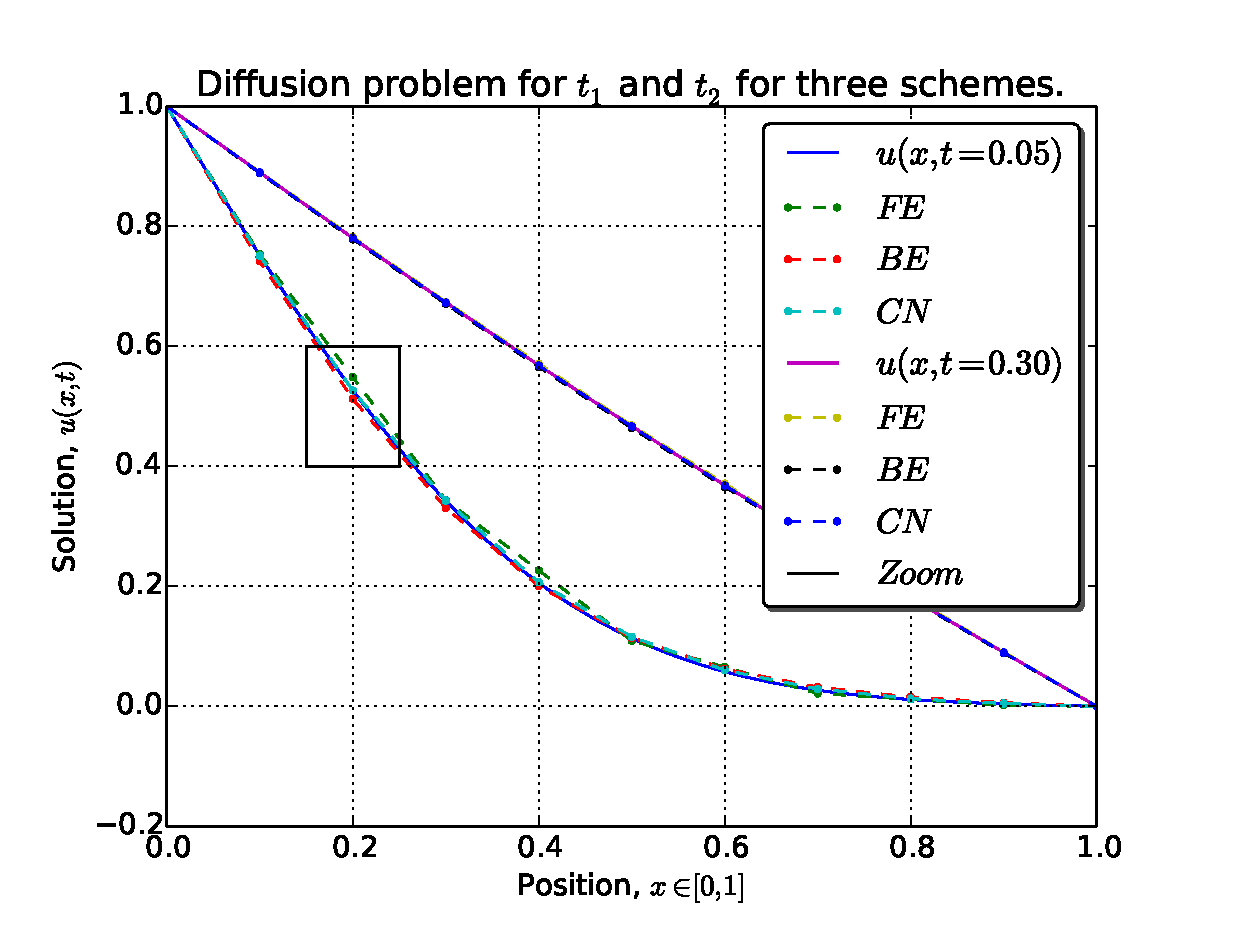
\includegraphics[width=0.5\textwidth]{Comparison_n10}}\quad
 \subfigure{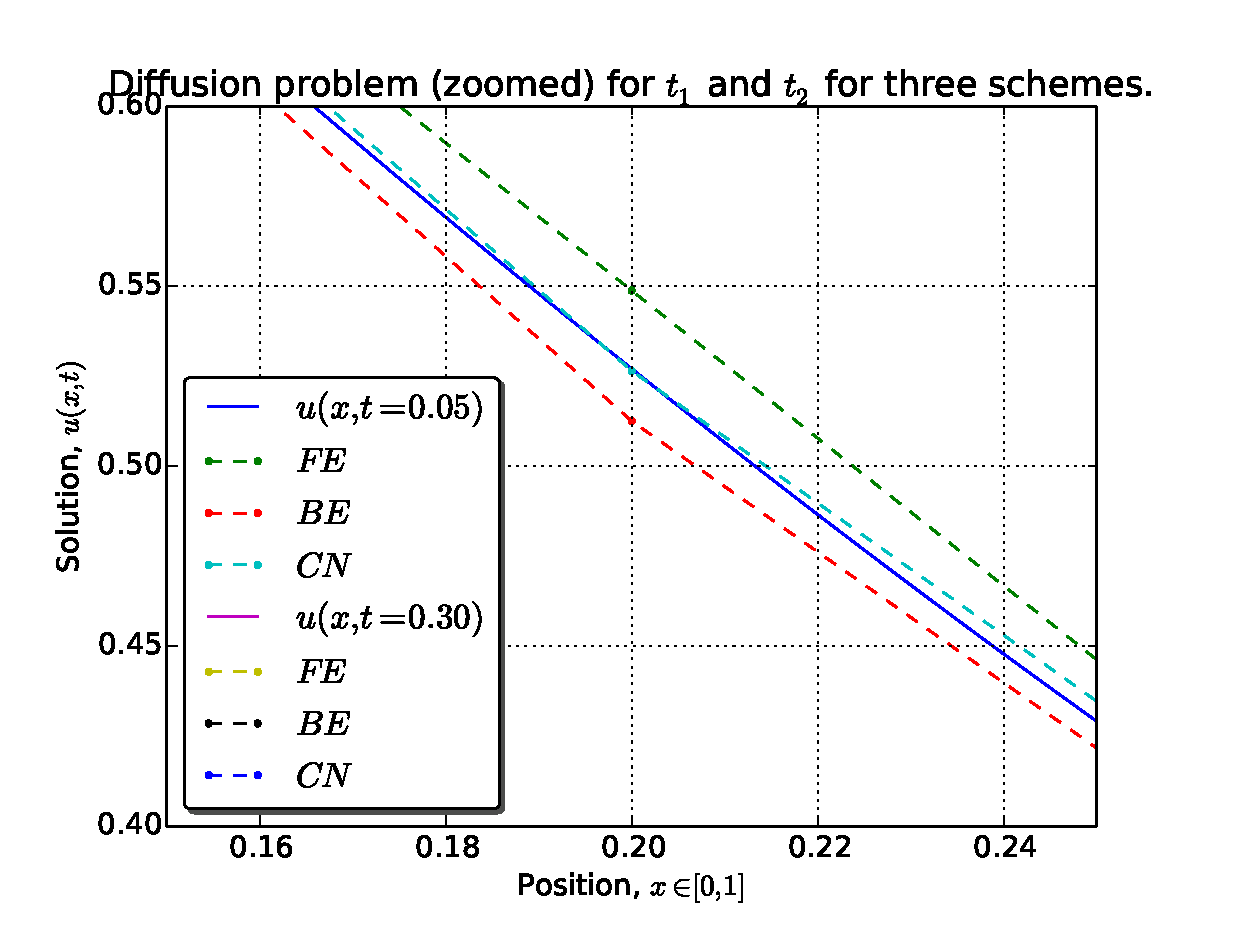
\includegraphics[width=0.5\textwidth]{Comparison_n10_zoom} }}
 \caption{Solutions found with the three direct solvers (FE – Forward Euler, BE – Backward Euler and CN – Crank-Nicolson) for $\Delta x = 0.1$ and 9 internal integration points at final times $t_1 = 0.05$ and $t_2 = 0.3$. The time step was chosen in accordance with the stability condition of the FE scheme, $\Delta t = 0.005$. The right figure is a zoom of the marked inset in the left figure. The analytical solution is shown for comparison. These figures were produced with the script \texttt{Project5\_d\_t1\_t2.py}. We included $500$ terms in the analytical solution before truncating the sum.}
\label{fig:Three_methods10}
\end{figure}

\begin{figure}[h!tb]
 \centering
 \mbox{\subfigure{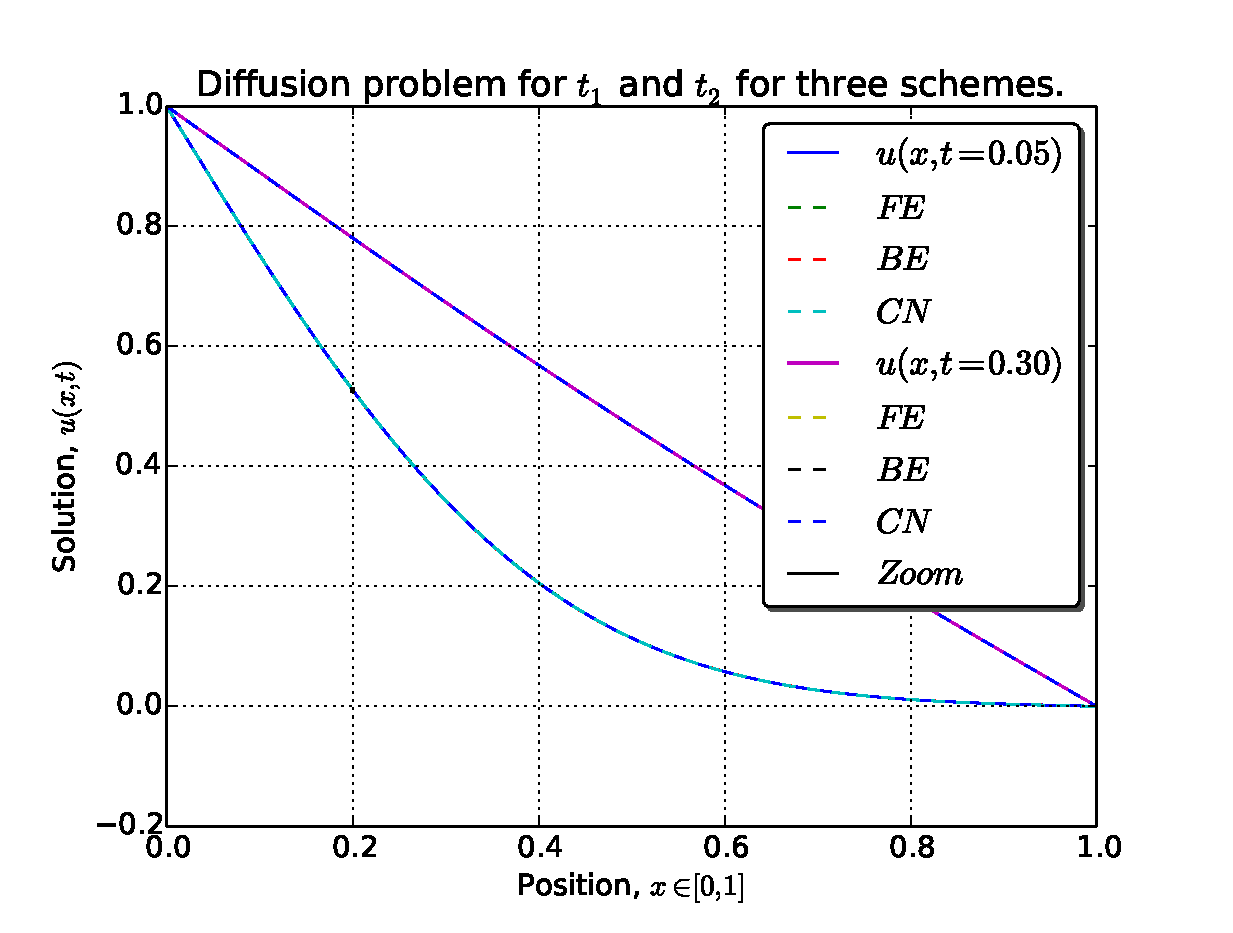
\includegraphics[width=0.5\textwidth]{Comparison_n100}}\quad
 \subfigure{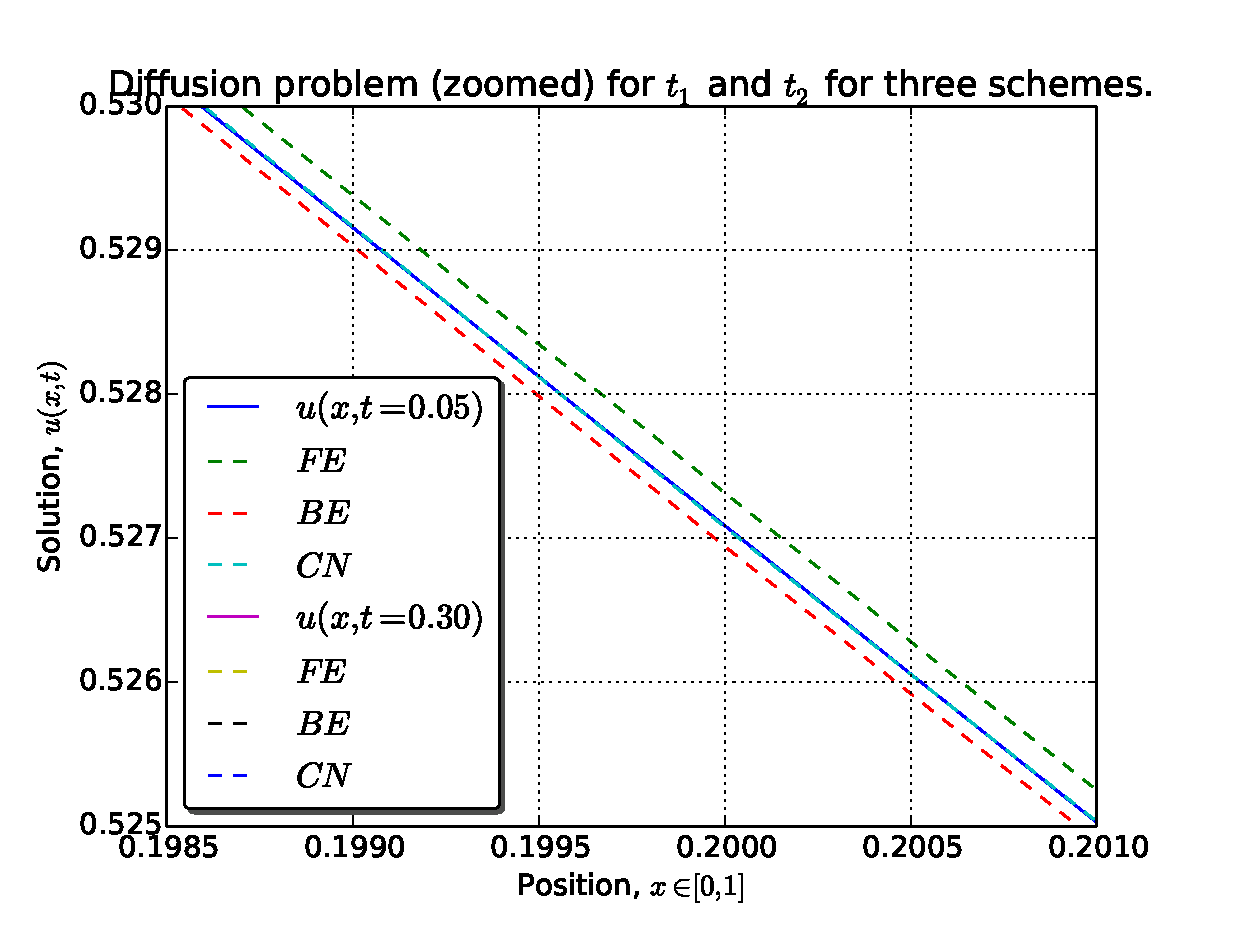
\includegraphics[width=0.5\textwidth]{Comparison_n100_zoom} }}
 \caption{Solutions found with the three direct solvers for $\Delta x = 0.01$ and 99 internal integration points at final times $t_1 = 0.05$ and $t_2 = 0.3$. Time step: $\Delta t = 0.00005$. The right figure is a zoom of the marked inset (very small) in the left figure. The analytical solution is shown for comparison (with $500$ terms before truncation). These figures were produced with the script \texttt{Project5\_d\_t1\_t2.py}.}
\label{fig:Three_methods100}
\end{figure}

\begin{figure}[h!tb]
 \centering\mbox{\subfigure{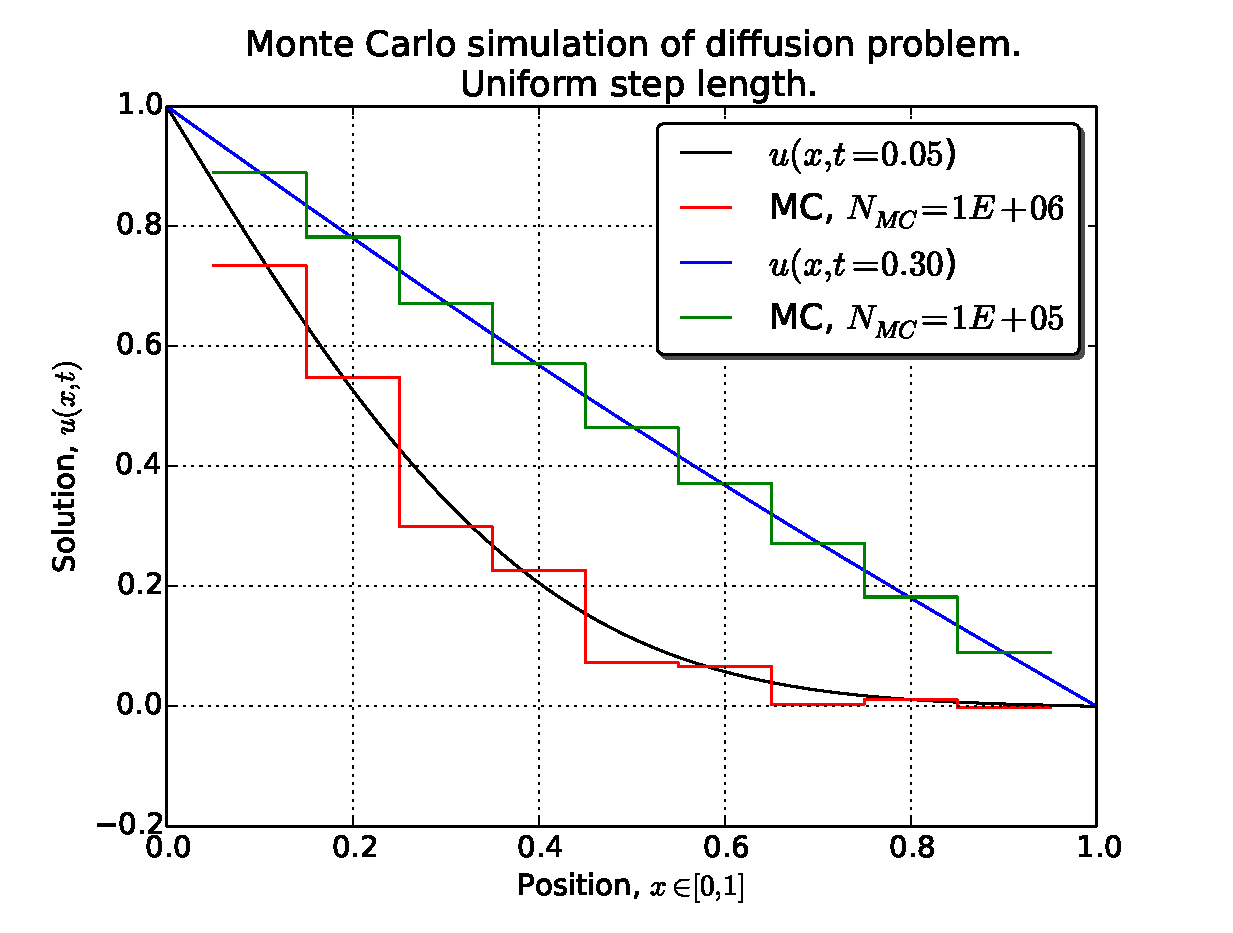
\includegraphics[width=0.5\textwidth]{MC_uniform_twoplot_T1}}\quad
 \subfigure{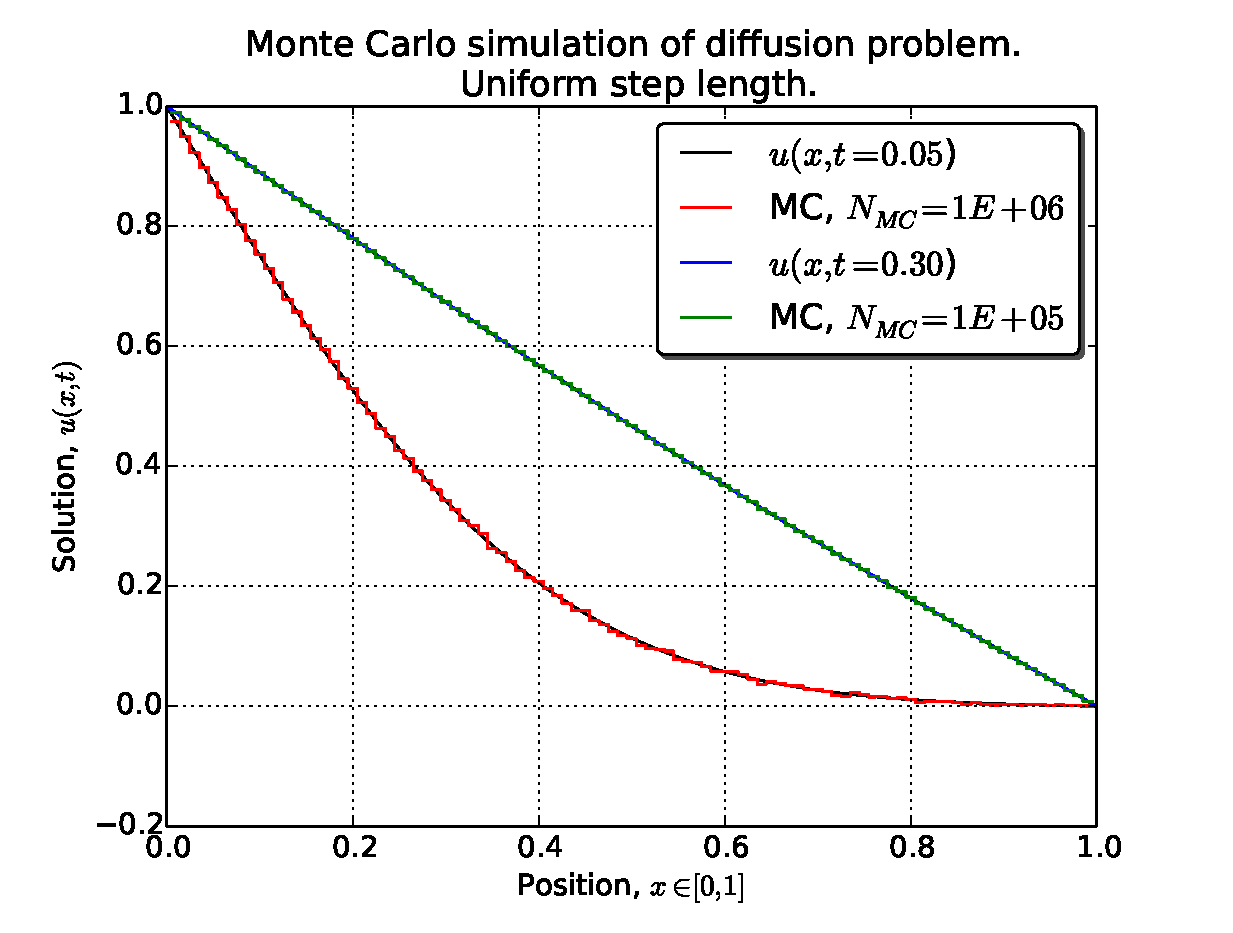
\includegraphics[width=0.5\textwidth]{MC_uniform_twoplot_T2} }}
 \caption{Random walk simulation with constant step length $\ell_0 = \sqrt{2\Delta t}$ and equal probability of moving left and right. $\Delta t = 0.005$ in the left figure and $\Delta t = 0.00005$ in the right figure. For the time $t_1 = 0.05$ we used \texttt{number\_walks} = $10^6$ and $10^5$ for $t_2 = 0.3$. The analytical solution is shown for comparison (with $500$ terms before truncation). Histograms are normalized in accordance with the discussion in section \ref{sec:MC_method}. These figures were produced with the script \texttt{Project5\_MCplotting1.py}.}
\label{fig:MC_uniform}
\end{figure}

\begin{figure}[h!tb]
 \centering
 \mbox{\subfigure{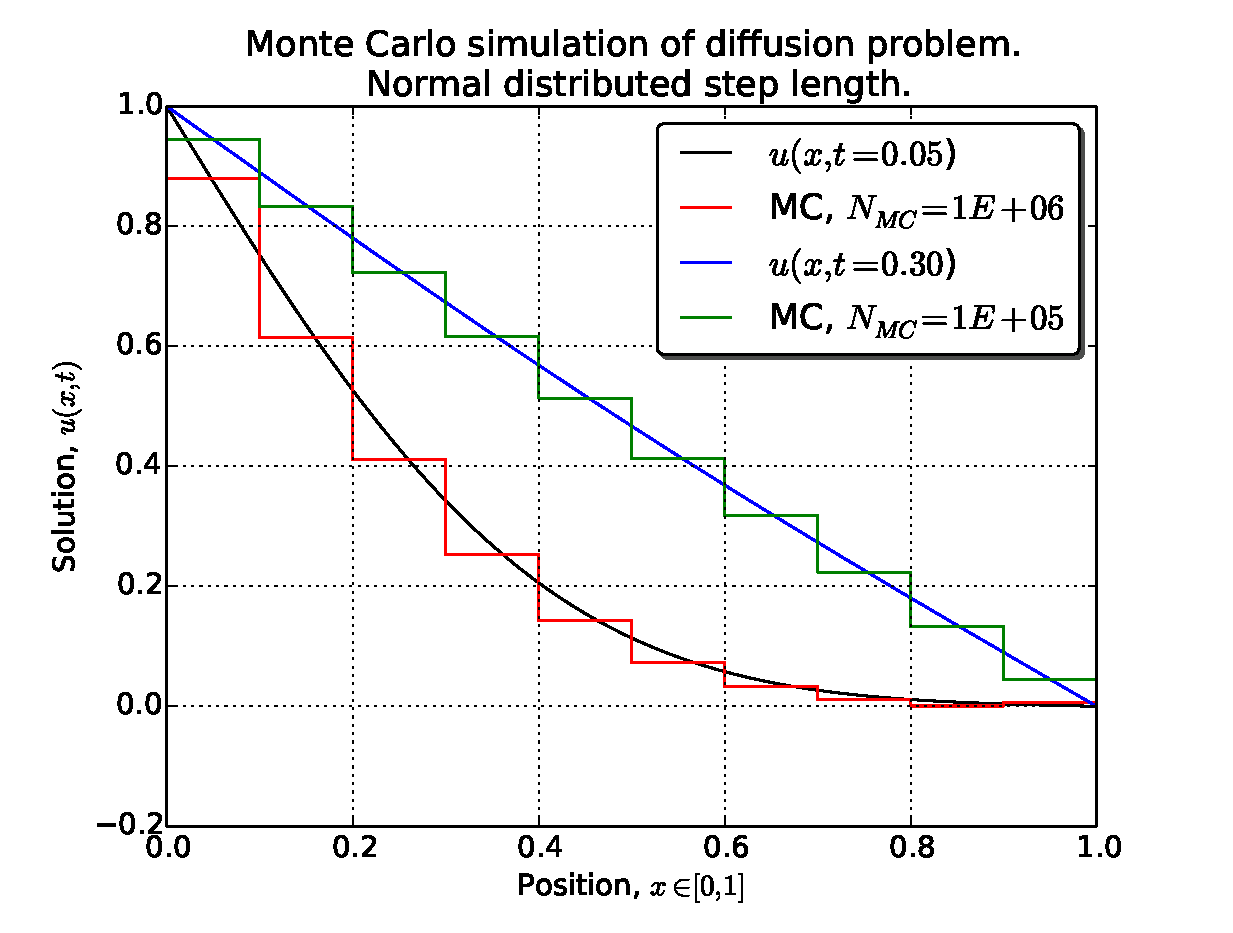
\includegraphics[width=0.5\textwidth]{MC_gaussian_twoplot_T1}}\quad
 \subfigure{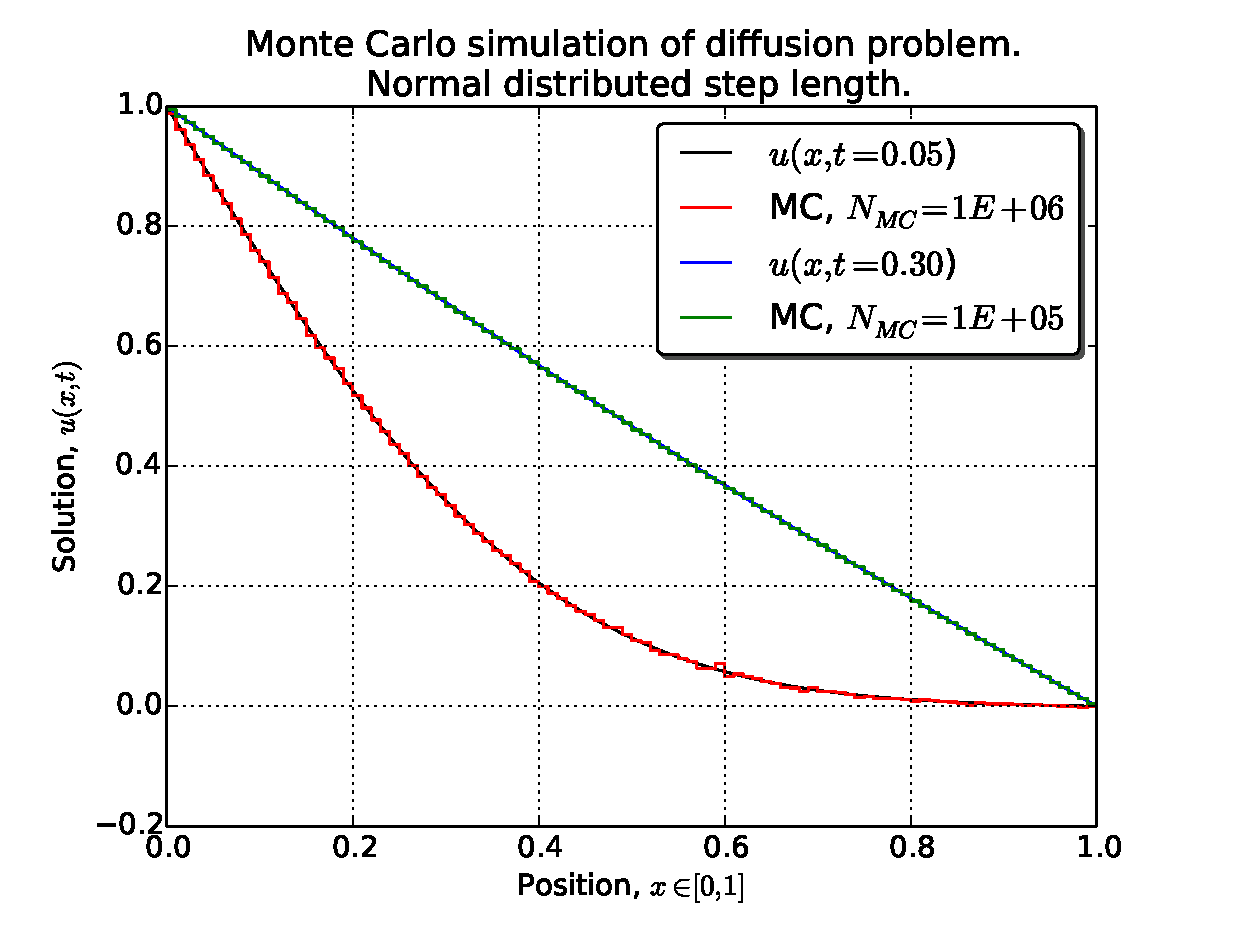
\includegraphics[width=0.5\textwidth]{MC_gaussian_twoplot_T2} }}
 \caption{Random walk simulation with varying step length $\ell_0 = \sqrt{2\Delta t}\xi$ with $\xi$ drawn from a normal distribution with mean 0 and standard deviation 1. $\Delta t = 0.005$ in the left figure and $\Delta t = 0.00005$ in the right figure. For the time $t_1 = 0.05$ we used \texttt{number\_walks} = $10^6$ and $10^5$ for $t_2 = 0.3$. The analytical solution is shown for comparison (with $500$ terms before truncation). Histograms are normalized in accordance with the discussion in section \ref{sec:MC_method}. These figures were produced with the script \texttt{Project5\_MCplotting2.py}.}
\label{fig:MC_gaussian}
\end{figure}

In the tables \ref{tab:Benchmark1}, \ref{tab:Benchmark2}, \ref{tab:Benchmark3} and \ref{tab:Benchmark4} we compare the numerical accuracy of all the five methods in terms of a 
spatial average of the absolute error in the calculation (the tables basically contain the same information as visualized in the plots). The final times in the tables are equal 
to the times used in all the plots, $t_1 = 0.05$ and $t_2 = 0.3$. These were found to be representative as the analytical solution is curved, but non-zero for all $x$ at
$t_1$, and at $t_2$ the solution is close to $u_s(x)$. The choice of $t_2$ is a compromise between the solution being close to $u_s(x)$, but time not too large for the
computation to be unreasonably slow (for the MC simulations). We chose to calculate

\begin{equation}
\epsilon(N_x,t) = \frac{1}{N_x}\sum_{i=1}^{N_x} \lvert u(x_i,t) - u'(x_i,t) \rvert
\label{eq:Mean_absolute_error}
\end{equation}

for all the methods, where $u'(x_i,t)$ refers to the numerical and $u(x_i,t)$ to the analytical solution at position $x_i$ and time $t$, and $N_x$ the number of grid points (or bins for the MC simulations) in $x$. The number $\epsilon(N_x,t)$ is used to reflect the quality of the numerical result\footnote{We could instead have calculated an average of the relative error, but for small times we risk a division of very small numbers since the analytical solution is close to zero in a large part of the interval. In addition, the absolute error (and not the relative error) should be compared with the standard deviation found in the Monte Carlo simulations.}. We also note here that $\Delta t$ was dictated by the strong stability condition of the Forward Euler scheme, $\Delta t \leq \Delta x^2 /2$. In these simulations we constantly put it equal to the upper limit, $\Delta t = \Delta x^2 /2$. In the appendix we provide an example of what happened to the solution if this condition was even slightly violated. We comment on the benchmark results and the plots in the next section.

\begin{table}[h!tb]
\begin{center}
\caption{Comparison of the five different methods for the final time $t_1 = 0.05$ with $\Delta t = 0.005$ and $\Delta x=0.1$ for the three direct solvers. $u'(x,t)$ refer to the numerical solution and the following abbreviations are used: FE – Forward Euler, BE – Backward Euler, CN – Crank-Nicolson, UMC – Uniform step Monte Carlo and GMC – Gaussian step Monte Carlo. The Monte Carlo calculations were done with \texttt{number\_walks} = $10^{6}$ and 9 or 10 bins as in the left of figure \ref{fig:MC_uniform} and \ref{fig:MC_gaussian}. The data in this table can be found in the files \texttt{Results\_n10.txt}, \texttt{Benchmark\_lowT1.txt} and \texttt{Benchmark\_lowT1\_gaussian.txt}.} 
\begin{tabular}{p{2cm} p{2cm} p{4cm} p{2.5cm}}
\toprule
Method & Calculation time, $T$ [s] & Average absolute error, $\frac{1}{N_x}\sum_i\lvert u(x_i,t) - u'(x_i,t) \rvert$ & Standard deviation (MC), $\sigma_t$ \\ \midrule
FE & $9\cdot 10^{-6}$ & $0.117808$ & N/A \\
BE & $1.0\cdot 10^{-5}$ & $0.143233$ & N/A \\
CN & $6\cdot 10^{-6}$ & $0.055469$ & N/A \\
UMC & $0.998$ & $0.020362$ & $0.025872$ \\
GMC & $2.16$ & $0.010392$ & $0.025454$ \\
\bottomrule
\end{tabular}
\label{tab:Benchmark1}
\end{center}
\end{table}

\begin{table}[h!tb]
\begin{center}
\caption{Comparison of the five different methods for the final time $t_1 = 0.05$ with $\Delta t = 0.00005$ and $\Delta x=0.01$ for the three direct solvers. The notation is otherwise the same as in table \ref{tab:Benchmark1}. Monte Carlo calculations were done with \texttt{number\_walks} = $10^{6}$ and 99 or 100 bins as in the right of figure \ref{fig:MC_uniform} and \ref{fig:MC_gaussian}. The data in this table can be found in the files \texttt{Results\_n100.txt}, \texttt{Benchmark\_lowT2.txt} and \texttt{Benchmark\_lowT2\_gaussian.txt}.} 
\begin{tabular}{p{2cm} p{2cm} p{4cm} p{2.5cm}}
\toprule
Method & Calculation time, $T$ [s] & Average absolute error, $\frac{1}{N_x}\sum_i\lvert u(x_i,t) - u'(x_i,t) \rvert$ & Standard deviation (MC), $\sigma_t$ \\ \midrule
FE & $0.000265$ & $0.001013$ & N/A \\
BE & $0.002495$ & $0.001901$ & N/A \\
CN & $0.003130$ & $0.000661$ & N/A \\
UMC & $68.4$ & $0.001961$ & $0.002506$ \\
GMC & $194$ & $0.001875$ & $0.002509$ \\
\bottomrule
\end{tabular}
\label{tab:Benchmark2}
\end{center}
\end{table}

\begin{table}[h!tb]
\begin{center}
\caption{Comparison of the five different methods for the final time $t_2 = 0.3$ with $\Delta t = 0.005$ and $\Delta x=0.1$ for the three direct solvers. The notation is otherwise the same as in table \ref{tab:Benchmark1}. Monte Carlo calculations were done with \texttt{number\_walks} = $10^{5}$ and 9 or 10 bins as in the left of figure \ref{fig:MC_uniform} and \ref{fig:MC_gaussian}. The data in this table can be found in the files \texttt{Results\_n10.txt}, \texttt{Benchmark\_highT1.txt} and \texttt{Benchmark\_highT1\_gaussian.txt}.} 
\begin{tabular}{p{2cm} p{2cm} p{4cm} p{2.5cm}}
\toprule
Method & Calculation time, $T$ [s] & Average absolute error, $\frac{1}{N_x}\sum_i\lvert u(x_i,t) - u'(x_i,t) \rvert$ & Standard deviation (MC), $\sigma_t$ \\ \midrule
FE & $0.000167$ & $0.003645$ & N/A \\
BE & $0.000120$ & $0.005997$ & N/A \\
CN & $0.000172$ & $0.001043$ & N/A \\
UMC & $2.28$ & $0.001614$ & $0.004338$ \\
GMC & $5.50$ & $0.002722$ & $0.004689$ \\
\bottomrule
\end{tabular}
\label{tab:Benchmark3}
\end{center}
\end{table}

\begin{table}[h!tb]
\begin{center}
\caption{Comparison of the five different methods for the final time $t_2 = 0.3$ with $\Delta t = 0.00005$ and $\Delta x=0.01$ for the three direct solvers. The notation is otherwise the same as in table \ref{tab:Benchmark1}. Monte Carlo calculations were done with \texttt{number\_walks} = $10^{5}$ and 99 or 100 bins as in the right of figure \ref{fig:MC_uniform} and \ref{fig:MC_gaussian}. The data in this table can be found in the files \texttt{Results\_n100.txt}, \texttt{Benchmark\_highT2.txt} and \texttt{Benchmark\_highT2\_gaussian.txt}} 
\begin{tabular}{p{2cm} p{2cm} p{4cm} p{2.5cm}}
\toprule
Method & Calculation time, $T$ [s] & Average absolute error, $\frac{1}{N_x}\sum_i\lvert u(x_i,t) - u'(x_i,t) \rvert$ & Standard deviation (MC), $\sigma_t$ \\ \midrule
FE & $0.001838$ & $0.000038$ & N/A \\
BE & $0.015674$ & $0.000059$ & N/A \\
CN & $0.019526$ & $0.000011$ & N/A \\
UMC & $186.9$ & $0.000493$ & $0.000434$ \\
GMC & $516.8$ & $0.000588$ & $0.000439$ \\
\bottomrule
\end{tabular}
\label{tab:Benchmark4}
\end{center}
\end{table}

\section{Discussion}
\label{sec:Discuss}
We divide the discussion and evaluation of results into two parts. The first part concerns the three direct solvers, the Forward Euler scheme, the Backward Euler scheme and the Crank-Nicoloson scheme. In the second part we discuss the uniform step and the Gaussian step Monte Carlo methods.

\subsection{Direct solvers}
The three direct solvers that were discussed in some detail in the earlier sections are seen to give quite satisfactory results in practice when comparing to the analytical 
solution. In figure \ref{fig:Three_methods10} we get the impression that only $9$ (internal) integration points is enough to make an overall good estimate. The situation in 
the zoomed inset is seen to be repeating for most times: the Forward Euler scheme is slightly over estimating, the Backward Euler scheme is slightly under estimating, while 
the Crank-Nicolson scheme lies somewhere in the middle. This last observation is quite intuitive as the latter scheme is an equally weighted sum of the two first schemes. \\

The computation times for these schemes can be seen from the tables to be typically of the same order, both for large times and small times and for both choices of $\Delta x$.
This can be understood from the algorithms given earlier. The Forward Euler scheme basically consists of one simple \texttt{for} loop over position for each time step; this 
means a number of FLOPS linear in $n$, $n$ being the number of mesh points. The Backward Euler scheme does, on the other hand, call the \texttt{tridiag()} function for each time 
step. This function also has a FLOP number linear in $n$ (basically some $8(n-1)$ FLOPS). The same goes for the Crank-Nicolson scheme, although it requires one additional loop 
for the computation of $\tilde{\boldsymbol{V}}_{j-1}$. In other words: All three methods should have almost constant ratios between the required number of FLOPS and hence almost
constant ratios of required computation time. \\

As was stated in section 2.3, the series of iterations $\boldsymbol{V}_i = A\boldsymbol{V}_{i-1} = A^{i}\boldsymbol{V}_0$ should converge to a definite value in the Backward Euler
and Crank-Nicholson schemes.
Studying the situation more carefully, we expand $\boldsymbol{V}_0$ in the eigenvectors of $A$, $\bo{a}_j$ with corresponding eigenvalues $\lambda_j$. Then
\begin{align}
 \lim\limits_{i\to\infty} A^{i}\bo{V}_0 &=  \lim\limits_{i\to\infty}A^i(v_1\bo{a}_1 + v_2\bo{a}_2 + \dots +v_n\bo{a}_n)\nonumber\\
  &=\lim\limits_{i\to\infty} (v_1\lambda_1^i\bo{a}_1 + v_2\lambda_2^i\bo{a}_2 + \dots + v_n\lambda_n^i\bo{a}_n) \nonumber\\
  &= \bo{0}
\end{align}
since all eigenvalues of $A$ are smaller than $1$. This is exactly what we see in Figures \ref{fig:Three_methods10} and \ref{fig:Three_methods100}: as the final time increases,
meaning number of time steps increases for a given $\Delta t$, 
the solution gets closer to the steady state $u_s(x,t)$, meaning $v(x,t)$ tends to zero. In the Forward Euler case we solved for $u(x,t)$ rather than $v(x,t)$. In doing so, we
added a constant vector for each iteration (equation (\ref{eq:Forward_Euler_matrix})), which means that the output will tend to the steady state solution rather than zero.
From the argument given above, it follows that for any process that can be described by a matrix equation with the matrix obeying (\ref{eq:Spectral_radius}) and with Dirichlet
boundary conditions, the solution will tend to zero as the number of iterations tends to infinity. \\

As the direct solvers all are based on Taylor methods and we know the exact solution, it would be interesting to calculate the local truncation error analytically from the Lagrange 
remainder formula. To actually use it to calculate an upper bound on the error did, however, prove difficult as we get sums of the form
\begin{equation}
 \sum\limits_{n=1}^\infty e^{-(n\pi)^2t}
\end{equation}
resembling a special case of the Jacobi theta function $\theta_3(0, e^{-\pi^2t})$. \\

Comparing the three direct solvers internally by judging from the results in table \ref{tab:Benchmark1}, \ref{tab:Benchmark2}, \ref{tab:Benchmark3} and \ref{tab:Benchmark4} we typically see that the Crank-Nicolson scheme gives an average absolute error almost one order of magnitude smaller than the other two. With no particular increase in computation time and no stability restrictions on the combination of $\Delta x$ and $\Delta t$, the Crank-Nicolson scheme should be characterized as the most satisfactory method among the three direct solvers for our one dimensional diffusion equation. \\

\subsection{Monte Carlo methods}
We argued for the elementary link between random walks and diffusion in section \ref{sec:RW}. A random walk offers a simplistic and intuitive implementation. The feature that made our implementation slightly more complex (as seen in listing \ref{lst:MC_uniform}) was how to take properly care of the absorbing boundaries. The \texttt{while} loop we set up was a way of handling a possible problem with to few final walkers and hence bad statistics. Without the loop, one must carefully increase the initial number of walkers with the final time in order to avoid loosing all walkers to the boundaries. To exemplify this, after 1000 time steps and $\Delta t = 0.00005$ with constant step length, we found that $1 015 731$ walkers escaped. Thus when we set \texttt{number\_walks} = $10^6$, the effective simulation is done with $2 015 731$ cycles, but with $10^6$ definite final positions. One might also use this as a point of objection. We are not really comparing the Monte Carlo methods on exactly the same statistical grounds. Another practical consequence of our choice is that the Monte Carlo simulations may take unreasonable long time to finish for large final times. This is just what our tables of results reflect. The computation time for the Monte Carlo simulations are of about 5 orders of magnitude greater than for the direct solvers. \\

Some simple tests were done during the implementation to check that the program was working properly. For instance, we checked that the initially drawn starting positions seemed to have the expected distribution given by $p(x)$ in equation (\ref{eq:MC_initial_dist}). We also saw that after one time step the walkers actually moved a distance $\ell_0$ by printing out walker positions and different messages inside each \texttt{if}-test (listing \ref{lst:MC_uniform}). \\

The program with normally distributed step length differs from the one with constant step lengths in some minor ways. The increase in computation time (typically by some factor between 2 and 3) must be almost solely due to the call on \texttt{gaussian\_deviate()} function. And with no particular gain of accuracy (rather a decrease for large times), this method does not contribute with any particular insights. Our measure of the statistical error $\sigma_t$ is satisfactory seen to be in the same order of magnitude as the absolute error. This can also be thought of as a simple test of our implementation. $\sigma_t$ is of course not expected to be exactly equal to the absolute error. One must keep in mind that it is an averaged quantity that approximates the standard deviation (in our case for $v(x,t)$). Another observation, which is generally consolidated by the table values, is that $\sigma_t$ should tend to zero for large final times since the number of escaped particles becomes large and the solution $v(x)$ itself also tends to zero. We also see (comparing for instance values in table \ref{tab:Benchmark1} and \ref{tab:Benchmark2}) how decreasing $\Delta x$ with a factor 10 reduces the absolute error and $\sigma_t$ with about the same factor. \\

Although these two methods based on random walks does not function as quick or particularly accurate solvers in (1+1) dimensions, they can be quite easily generalized to simulate a system where the diffusion constant is a function of position $D = D(x)$ \cite{Farnell}. In addition, we recall from project 3 – where we solved a six-dimensional integral with Monte Carlo methods – that Monte Carlo methods typically gives better results when the number of spatial dimensions become large. This is because the statistical error of Monte Carlo methods scale independently of the number of dimensions. The errors of finite difference methods do on the other hand depend on the number of dimensions. It should, based on what we have discussed in the previous paragraphs, and by comparing table values, be fair to conclude that the Crank-Nicolson scheme is the fastest and most accurate solver (without a huge penalty in large number of FLOPS) for the (1+1)-dimensional diffusion equation.

\section{Conclusion}
We started this project with a discussion of the diffusion equation in one spatial dimension. We restricted ourselves to boundary conditions that could corresponded to a 
release of transmitter molecules from the presynaptic cleft and absorption at the postsynaptic cleft. We derived a closed form analytical solution – it later functioned as 
our main reference when checking the numerical implementations. After seeing how random walks are intrinsically linked to diffusion, we spent some time on presenting three 
direct solvers, their stability conditions, truncation errors and implementations. Two intuitive Monte Carlo based methods were also presented and implemented. These methods
were seen to result in somewhat slow computations and did not in general introduce any particular gain of accuracy as compared to the direct solvers. With this said, we met 
several interesting challenges and aspects during the implementation, and they demanded to a greater extent than the direct solvers algorithmic thinking. \\

Based on numerical accuracy and computation time we conclude that in the case of the (1+1)-dimensional diffusion equation, the Crank-Nicolson scheme offered the overall best results. It is expected that this conclusion would be altered if we were to do the same comparison in higher spatial dimensions where Monte Carlo based methods previously have shown to be superior.

\section{Appendix}
In figure \ref{fig:Dt_violation} we provide an example of what happens with the solutions found with the three direct solvers when the stability condition for the Forward Euler scheme is slightly violated. The figure was produced with $\Delta t = 0.502 \Delta x^2$ (an even smaller violation gave clearly visible effects, but our choice was found to illustrate the problems with the explicit scheme without total domination over the solutions from the other schemes). In the figure one can see how only the Forward Euler scheme gives oscillating and worthless results after only some few time steps. The implicit scheme and the Crank-Nicolson scheme are still stable and can not be visually separated from the exact solution without zooming. This is in perfect accordance with the stability conditions we derived earlier and can be seen as a simple test of the developed programs.

\begin{figure}[h!tb]
 \centering
 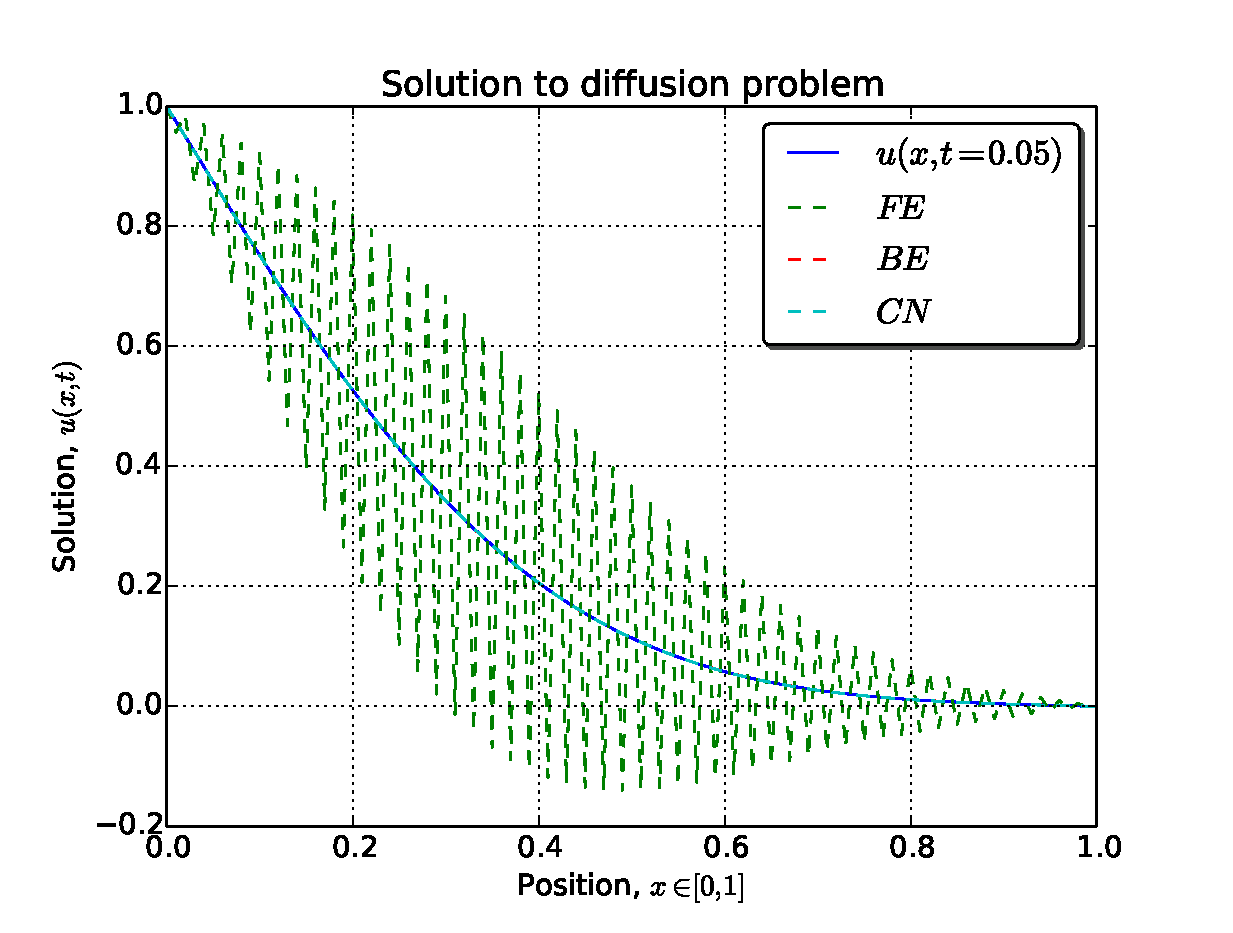
\includegraphics[width=0.7\textwidth]{Violate_Dt}
 \caption{Solutions found with the three direct solvers (FE – Forward Euler, BE – Backward Euler and CN – Crank-Nicolson) for $\Delta x = 0.01$ and 99 internal integration points at (absolute) time $t_1 = 0.05$. We put $\Delta t = 0.502 \Delta x^2$ when producing this figure, i.e. a slight violation of the stability criterion for the Forward Euler scheme. This figure was produced with the script \texttt{Project5\_e.py}. }
\label{fig:Dt_violation}
\end{figure}

\bibliography{References_pro5}

\section*{Code listing}
A list of all the codes files developed during the work with this project is given below. The source files and all the benchmark calculations can be found at the github domain mentioned in the beginning of this document. \\

\begin{itemize}
\item Codes for part d and e: \{\texttt{Project5\_d.cpp}, \texttt{Project5\_d\_t1\_t2.py}\}

\item Codes for part f: \{\texttt{Project5\_f.cpp}, \texttt{Project5\_f.py}, \texttt{Project5\_MCplotting1.py}\}

\item Codes for part g: \{\texttt{Project5\_g.cpp}, \texttt{Project5\_g.py}, \texttt{Project5\_MCplotting2.py}\}

\item Codes for the appendix (violation of the stability condition): \{\texttt{Project5\_e.py}\}
\end{itemize}

 %\begin{equation}
 %\delta a = \delta \gamma\cos{\gamma}
%\label{eq:aksel_1_usikker}
%\end{equation}
 
 %\begin{table}[h!tb]
%\begin{center}
   %\begin{tabular}{ | p{2cm} | p{2cm} | p{3cm} |}
    %\hline
     %& $x_i$ [mm] & $\delta x_i$ [mm] \vspace{2 mm} \\ \hline
     %$l_a$ & 708 & 0   \\ 
     %$dl_s$ & 0 & 0.5  \\ 
     %$\sqrt{n}\cdot dl_l$ & 0 & $\sqrt{3}\cdot0.5 =0.87$  \\ 
     %$dl_m$ & 0 & $0.1\cdot\frac{708}{100} = 0.71$ \vspace{2 mm} \\ \hline
     %&$\sum_i x_i$ & $\sqrt{\sum_i \delta x_i}$  \\ 
     %& 708 & 1.12 \\ \hline
    %\end{tabular}
%\end{center}
%\caption{Måling av $x$ med målestokk. Til gjeldende antall siffer: $x = (708 \pm 1)$ mm.}
%\end{table}
 
 %\begin{figure}[h!tb]
 %\centering
 %\mbox{\subfigure{\includegraphics[width=2.7in]{kjent_vinkel_skraaplan}}\quad
 %\subfigure{\includegraphics[width=2.7in]{kjent_vinkel_skraaplan_linreg} }}
 %\caption{Til venstre: Hastighet som funksjon av tid mens bilen trillet langs skråplanet. Til høyre: Lineær regresjon på partiet der hastigheten øker jevnt.}
%\end{figure}

%\begin{figure}[h!tb]
 %\centering
 %includegraphics[width=2.7in]{Raynold_Rayleigh}
 %\caption{Plott av data fra tabell 2, dvs. Raynoldstallet plottet mot henholdsvis Rayleigh- og Stokes-koeffisientene for de ulike kombinasjonene av ballonger og vekter.}
%\end{figure}

%%% Eksempel på linjert matematikk med tall for hver linje %%%
%\begin{align}
%   n &=  \int_0^\infty n\left( \frac{1}{2\pi mkT} \right)^{3/2} e^{-\frac{p^2}{2mkT}}4\pi p^2 \hspace{1mm} dp \\
%  &= 4\pi n\left( \frac{1}{2\pi mkT} \right)^{3/2}\int_0^\infty e^{-x} \underbrace{2mkTx}_{p^2} \underbrace{\frac{mkT}{\sqrt{2mkTx}}dx}_{dp} \\
%  &= 4\pi n \left[ \frac{1}{2\pi mkT}\cdot (2mkT)^{1/3} \cdot (mkT)^{2/3} \right]^{3/2}\underbrace{\int_0^{\infty} x^{1/2}e^{-x} \hspace{1mm} dx}_{\frac{\sqrt{\pi}}{2}} \\
%  &= 4\pi n \left[ \frac{1}{2^{2/3}\pi} \right]^{3/2}\frac{\sqrt{\pi}}{2} \\
%  &= 2\pi^{3/2}n\cdot \frac{1}{2\pi^{3/2}} = n
%\end{align}

%%% Eksempel på listing av kode %%%
%\lstset{language=python,caption={Program for å numerisk bekrefte at $PV=NkT$.}}
%\begin{lstlisting}
%# OBLIG 11; Ideal gas law
%def find_P(T,N):
%    u = 1.66054*10**(-27)          # [kg]
%    m = u*1.0079                   # [kg], mass of hydrogen atom
%    dt = 10**(-9)                  # [s]
%    A = 6*B_wall**2                # [m^2]

%    sigma = sqrt(k*T/m)
%    v = zeros((N,3))
%    r = zeros((N,3))

%    F = 0
%    for i in xrange(N):
%        v[i] = array([rn.gauss(0,sigma),rn.gauss(0,sigma),rn.gauss(0,sigma)])
%        r[i] = array([rn.uniform(0,B_wall),rn.uniform(0,B_wall),rn.uniform(0,B_wall)])
%        p = m*v[i]
%        for j in xrange(3):
%           if (abs(v[i,j])*dt >= B_wall-r[i,j]):
%              F += 2*abs(p[j])/dt
%    P = F/A
%    return P
%\end{lstlisting}


%%% Eksempel på tabelloppsett %%%
%\begin{center}
   %\begin{tabular}{ | p{2cm} | p{3cm} | p{3cm} |}
    %\hline
    %Event A: & $x_A=0$ & $t_A=0$ \vspace{2 mm} \\ \hline
    %& $x_A^{'}=0$ & $t_A^{'}=0$ \vspace{2 mm}  \\ \hline
    %Event B: & $x_B=L_0$ & $t_B=L_0$ \vspace{2 mm} \\ \hline
    % & $x_B^{'}=L_0\gamma(1-v)$ & $t_B^{'}=L_0\gamma(1-v)$ \vspace{2 mm}  \\ \hline
    %Event C: & $x_C=vL_0$ & $t_C=L_0$ \vspace{2 mm} \\ \hline
     %& $x_C^{'}=0$ & $t_C^{'}=\frac{L_0}{\gamma}$ \vspace{2 mm}  \\ \hline
    %\end{tabular}
%\end{center}


%%% Eksempel på inkludering av figur %%%
%\begin{figure}[h!tb]
 %\centering
 %\includegraphics[width=\textwidth]{star4}
%\end{figure}

\end{document}
